% MS Project Report: Multi-Agent Powerplant Monitoring System
% TGS Format: 8.5" x 11", 1" margins, 12pt Times, double-spaced

\documentclass[12pt,letterpaper]{report}
\usepackage[utf8]{inputenc}
\usepackage[T1]{fontenc}
\usepackage{mathptmx}  % Times New Roman
\usepackage[margin=1in]{geometry}
\usepackage{setspace}
\doublespacing

\usepackage{graphicx}
\graphicspath{{../evaluation/report/}}
\usepackage{booktabs}
\usepackage{tikz}
\usetikzlibrary{shapes,arrows,positioning,fit,calc}
\usepackage{hyperref}
\usepackage{amsmath}
\usepackage{listings}
\usepackage{xcolor}
\usepackage{caption}
\usepackage[numbers]{natbib}  % IEEE-style numbered refs [1], [2]
\usepackage{seqsplit}  % allow \texttt to break long identifiers at any character

% Code listing style
\lstset{
  basicstyle=\ttfamily\small,
  breaklines=true,
  frame=single,
  backgroundcolor=\color{gray!10},
  showspaces=false,
  showstringspaces=false,
}

% Hyperref
\hypersetup{colorlinks=true, linkcolor=blue, citecolor=blue, urlcolor=blue}

% Page number: upper right, 3/4" from top
\usepackage{fancyhdr}
\pagestyle{fancy}
\fancyhf{}
\renewcommand{\headrulewidth}{0pt}
\fancyhead[R]{\thepage}
\fancypagestyle{plain}{\fancyhead[R]{\thepage}}
\setlength{\headheight}{14.5pt}
% Allow line breaks inside long \texttt to avoid overflow
\let\oldtexttt\texttt
\renewcommand{\texttt}[1]{\oldtexttt{\seqsplit{#1}}}
% Reduce overfull hbox: let LaTeX stretch more when needed
\setlength{\emergencystretch}{3em}
\sloppy

\begin{document}

% ========== Title Page (no page number) ==========
\thispagestyle{empty}
\begin{center}
\vspace*{0.75in}
{\Large \textbf{NORTHWESTERN UNIVERSITY}}

\vspace{1in}
{\Large Multi-Agent Powerplant Monitoring System: Real-Time Anomaly Detection, Root Cause Analysis, and Human-in-the-Loop Review}

\vspace{0.75in}
{\large A PROJECT REPORT}

\vspace{0.4in}
SUBMITTED TO THE GRADUATE SCHOOL\\
IN PARTIAL FULFILLMENT OF THE REQUIREMENTS\\
for the degree\\
\textbf{MASTER OF SCIENCE}\\
\textbf{Computer Engineering}

\vspace{0.75in}
By\\
\textbf{Haoji Bian}

\vspace{0.75in}
EVANSTON, ILLINOIS\\
February 2026
\end{center}
\newpage

% ========== Abstract ==========
\setcounter{page}{2}
\chapter*{Abstract}
\addcontentsline{toc}{chapter}{Abstract}

This report presents the design, implementation, and evaluation of a multi-agent system for powerplant asset monitoring. The system consists of four agents: a Monitor (Agent A) that detects anomalies in real-time telemetry using threshold-based methods, a Diagnosis agent (Agent B) that performs root cause analysis via LangChain ReAct with rule retrieval, a Ticket agent (Agent C) that creates review requests, and a Review agent (Agent D) that provides a human-in-the-loop interface with RAG-assisted chat. All agents communicate over MQTT. A physics-based simulator with fault injection (bearing wear, clogging, valve stuck, sensor drift, noise burst) enables reproducible evaluation. On 390 scenario runs, the system achieves 44.9\% alert detection rate, 81.1\% diagnosis accuracy, 83.3\% fault scenario detection rate, and 11.9\% healthy false positive rate. Bearing wear and valve stuck scenarios achieve 100\% diagnosis accuracy; clogging and sensor override show lower accuracy. The report concludes with a discussion of limitations and future work.

\newpage

% ========== Table of Contents ==========
\tableofcontents
\newpage

% ========== List of Figures ==========
\listoffigures
\addcontentsline{toc}{chapter}{List of Figures}
\newpage

% ========== List of Tables ==========
\listoftables
\addcontentsline{toc}{chapter}{List of Tables}
\newpage

% ========== Acknowledgments ==========
\chapter*{Acknowledgments}
\addcontentsline{toc}{chapter}{Acknowledgments}

I would like to thank my advisor, Professor Qi Zhu, for his guidance and support throughout this project. I am grateful to Simon Zhan, my PhD mentor, for his valuable advice and feedback. I also thank David Zaretsky, Director of the MS Program in Computer Engineering, for his support of the graduate program.

\newpage

% ========== Chapter 1: Introduction ==========
\chapter{Introduction}
\label{ch:intro}

\section{Motivation and Problem Statement}

Industrial Internet of Things (IoT) asset monitoring requires real-time processing of sensor telemetry, timely fault detection, and interpretable root cause analysis (RCA) to support maintenance decisions. Traditional approaches often rely on black-box machine learning models that lack transparency, or on manual ticket creation that delays response. Furthermore, safety-critical applications demand human-in-the-loop review before automated actions are executed.

This report addresses the following research question: Can a multi-agent system combining rule-based anomaly detection, large language model (LLM)-based diagnosis with ReAct (Reasoning and Acting) reasoning, and retrieval-augmented generation (RAG) achieve reliable fault diagnosis with interpretable evidence?

\section{Objectives}

The primary objectives of this project are:

\begin{enumerate}
\item Design and implement a four-agent pipeline: Monitor $\rightarrow$ Diagnosis $\rightarrow$ Ticket $\rightarrow$ Review, with each agent fulfilling a distinct role.
\item Integrate threshold-based anomaly detection, ReAct-based diagnosis with tool use, and RAG for context retrieval in the review interface.
\item Evaluate detection rate, diagnosis accuracy, and healthy false positive rate on fault-injected scenarios using a reproducible evaluation framework.
\end{enumerate}

\section{Contributions}

The main contributions of this report are:

\begin{itemize}
\item An end-to-end multi-agent architecture for powerplant monitoring, with agents communicating via MQTT (Message Queuing Telemetry Transport).
\item A rule-plus-LLM hybrid diagnosis approach with evidence traceability through ReAct reasoning and tool calls.
\item A reproducible evaluation framework with fault injection and scenario-driven testing.
\end{itemize}

\section{Report Organization}

Chapter~\ref{ch:background} reviews related work in industrial IoT, anomaly detection, root cause analysis, multi-agent systems, and RAG. Chapter~\ref{ch:design} presents the system design, including architectural background, LLM/ReAct/RAG design, and component specifications. Chapter~\ref{ch:impl} describes the implementation. Chapter~\ref{ch:eval} presents the evaluation results. Chapter~\ref{ch:conclusion} concludes and outlines future work.

% ========== Chapter 2: Background ==========
\chapter{Background and Related Work}
\label{ch:background}

\section{Industrial IoT and Asset Monitoring}

Industrial IoT enables real-time sensor streams from physical assets such as pumps, motors, and bearings~\cite{lee2015cps,rahman2022deep,li2021intelligent}. Lee et al.~\cite{lee2015cps} describe a cyber-physical systems architecture for Industry 4.0, where manufacturing systems integrate sensing, computation, and actuation for predictive maintenance. Wang et al.~\cite{rahman2022deep} survey deep-learning-enabled predictive maintenance in industrial IoT, highlighting methods for anomaly detection, remaining useful life estimation, and fault prognosis. Zhu et al.~\cite{li2021intelligent} provide a comprehensive survey of intelligent predictive maintenance for industrial equipment, covering data-driven and model-based approaches.

SCADA (Supervisory Control and Data Acquisition) systems and predictive maintenance frameworks aim to detect anomalies before failures occur, reducing unplanned downtime and maintenance costs. Common fault types in rotating machinery include bearing wear, pipe clogging, valve malfunction, and sensor drift. These faults manifest as distinct patterns in telemetry signals---e.g., bearing wear increases vibration and temperature; clogging reduces flow and increases pressure differential---which motivates the design of multi-signal detection and diagnosis pipelines.

\section{Anomaly Detection}

Anomaly detection identifies patterns that do not conform to expected behavior~\cite{chandola2009anomaly,ahmed2016survey}. Chandola et al.~\cite{chandola2009anomaly} provide a broad survey of anomaly detection techniques, categorizing them into statistical, machine learning, and hybrid approaches. Ahmed et al.~\cite{ahmed2016survey} focus on network anomaly detection but discuss principles applicable to general time-series data.

Statistical methods such as Z-score and threshold-based detection with sliding windows are widely used for real-time telemetry. These methods are interpretable, require minimal training data, and can be tuned for specific signals. Threshold-based detection checks whether a signal exceeds a configured limit; duration checks help avoid false positives from transient spikes. Slope-based detection identifies trends (e.g., rising temperature over time) that may indicate gradual degradation.

Machine learning approaches, including deep learning, offer flexibility but often sacrifice interpretability. Deep models can learn complex patterns from raw or aggregated data but may require large labeled datasets and lack transparency for safety-critical applications. Hybrid approaches that combine rule-based thresholds with learned models are increasingly explored for industrial IoT monitoring.

In industrial settings, baseline or normal-profile modeling establishes expected ranges for each signal under healthy conditions~\cite{li2021intelligent}. A sliding-window buffer maintains recent samples for computing statistics (mean, variance, slope) over short intervals. Duration checks require that a threshold violation persist for a minimum time before triggering an alert, reducing false positives from transient noise. Wang et al.~\cite{rahman2022deep} note that combining multiple detection criteria---e.g., threshold, slope, and duration---improves robustness for real-time telemetry streams.

\section{Root Cause Analysis}

Root cause analysis (RCA) links observed symptoms to underlying faults~\cite{isermann2006fault,yin2012comparison}. Isermann~\cite{isermann2006fault} provides a foundational treatment of fault-diagnosis systems, from fault detection to fault tolerance. Yin et al.~\cite{yin2012comparison} compare data-driven fault diagnosis methods on the Tennessee Eastman benchmark, demonstrating trade-offs between model-based and data-driven approaches.

Rule-based systems provide interpretability: domain experts encode symptom-to-fault mappings in rules or decision trees, enabling traceable diagnoses. Data-driven methods, such as support vector machines or neural networks, can capture complex patterns but may be less interpretable. Zhang et al.~\cite{zhang2009fault} apply fault tree analysis for power electronic systems; Chen and Patton~\cite{chen1999robust} discuss robust model-based fault diagnosis for dynamic systems.

Recent work on LLM-based reasoning with tool use~\cite{yao2023react,schick2023toolformer} enables multi-step inference with evidence traceability. Yao et al.~\cite{yao2023react} introduce ReAct: interleaving reasoning (Thought) and acting (tool calls) in language models. Schick et al.~\cite{schick2023toolformer} show that language models can learn to use tools for external knowledge retrieval. This paradigm is well-suited for diagnosis: the LLM can query rules, telemetry, and past alerts, then produce structured output with root cause and evidence.

Beyond ReAct, chain-of-thought prompting and tree-based search extend LLM reasoning. Yao et al.~\cite{yao2023tot} propose Tree of Thoughts, which explores multiple reasoning paths and backtracks when a path fails, enabling deliberate problem solving. Such methods complement tool use by improving the quality of multi-step inference when the solution space is large or ambiguous.

\section{Multi-Agent Systems}

Multi-agent systems coordinate autonomous entities through message passing and pub/sub architectures~\cite{wooldridge2009multiagent,russell2020aima}. Wooldridge~\cite{wooldridge2009multiagent} defines agents as autonomous entities that perceive their environment and act to achieve goals. Russell and Norvig~\cite{russell2020aima} discuss agent architectures, including reactive agents and agents with internal state.

In industrial IoT, a multi-agent design allows separation of concerns: one agent monitors telemetry, another diagnoses faults, another creates tickets, and another supports human review. This modularity improves scalability and fault isolation---a failure in one agent does not necessarily halt the entire pipeline.

MQTT (Message Queuing Telemetry Transport) is a lightweight publish-subscribe protocol suitable for industrial IoT~\cite{oasis2019mqtt,hussain2021mqtt}. OASIS~\cite{oasis2019mqtt} defines the MQTT v3.1.1 standard. Recent work such as MQTT-I~\cite{hussain2021mqtt} analyzes MQTT deployments and protocol-level issues, including end-to-end data integrity when brokers may not be fully trusted. Topics such as \texttt{telemetry/\{asset\_id\}} and \texttt{alerts/\{asset\_id\}} enable loose coupling between agents.

\section{Retrieval-Augmented Generation}

RAG enriches language model context with retrieved documents~\cite{lewis2020rag,borgeaud2022retrieving}. Lewis et al.~\cite{lewis2020rag} introduce retrieval-augmented generation for knowledge-intensive NLP tasks, combining a dense retriever with a sequence-to-sequence model. Borgeaud et al.~\cite{borgeaud2022retrieving} demonstrate that retrieving from large external corpora improves language model performance on factual and reasoning tasks.

Vector search and semantic retrieval support domain knowledge integration for diagnosis and review. Embedding models (e.g., sentence-transformers) map text to dense vectors; similarity search retrieves relevant past diagnoses, rules, or alerts. This enables the review agent to answer questions such as ``What similar past diagnoses exist?'' or ``Which rules apply to this symptom?'' without relying solely on the LLM's parametric knowledge.

RAG is particularly valuable when domain knowledge is dynamic (e.g., new rules or feedback) or when the model's training cutoff predates recent events. For powerplant monitoring, indexing alerts, diagnoses, rules, feedback, and chat messages into a vector store allows the agent to ground its responses in context-specific evidence.

Practical RAG implementations rely on embedding models and vector indexes. Reimers and Gurevych~\cite{reimers2019sentence} introduce Sentence-BERT, which produces semantically meaningful sentence embeddings via siamese BERT networks; the sentence-transformers library provides pre-trained models such as all-MiniLM-L6-v2 (384 dimensions) for efficient retrieval. Vector databases store embeddings and support similarity search; sqlite-vec~\cite{sqlitevec2024} extends SQLite with vector similarity search, enabling lightweight, file-based RAG without a separate vector store service.

\section{Vision Language Models}

Vision language models (VLMs) extend LLMs to process both images and text, enabling multimodal reasoning over visual inputs~\cite{li2022blip,liu2023llava,zhang2024mmllms}. Li et al.~\cite{li2022blip} present BLIP for unified vision-language understanding and generation; Liu et al.~\cite{liu2023llava} introduce visual instruction tuning for aligning vision encoders with language models. Zhang et al.~\cite{zhang2024mmllms} survey recent advances in multimodal large language models. In industrial monitoring, VLMs can analyze visualization images (e.g., 3D pump renderings or dashboard screenshots) and produce textual descriptions or anomaly reports, complementing sensor-based diagnosis with visual evidence.

% ========== Chapter 3: System Design ==========
\chapter{System Design}
\label{ch:design}

\section{Overview}

The system comprises five main components: a Simulator, Agent A (Monitor), Agent B (Diagnosis), Agent C (Ticket), and Agent D (Review). Data flows from telemetry to alerts, diagnosis, tickets, and human feedback. Figure~\ref{fig:architecture} shows the high-level architecture. The Simulator generates telemetry and publishes to MQTT; Agent A detects anomalies and publishes alerts; Agent B diagnoses root causes via ReAct and publishes diagnosis reports; Agent C creates review requests; Agent D provides the human-in-the-loop interface with a React frontend, RAG-assisted chat, and approve/reject workflow.

\begin{figure}[htbp]
\centering
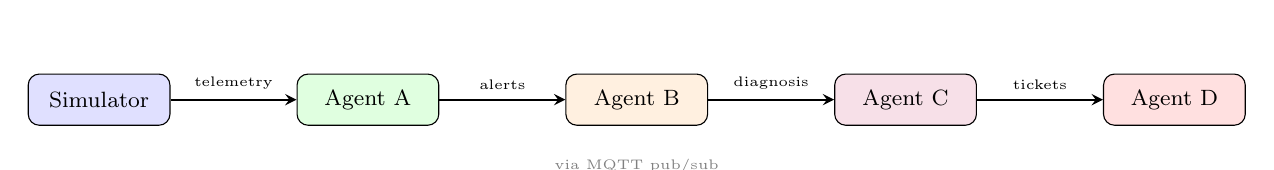
\begin{tikzpicture}[
  node distance=0.6cm,
  box/.style={rectangle, draw, rounded corners, minimum width=1.8cm, minimum height=0.65cm, align=center, font=\footnotesize},
  arrow/.style={->, >=stealth, thick}
]
  \node[box, fill=blue!12] (sim) {Simulator};
  \node[box, fill=green!12, right=1.6cm of sim] (a) {Agent A};
  \node[box, fill=orange!12, right=1.6cm of a] (b) {Agent B};
  \node[box, fill=purple!12, right=1.6cm of b] (c) {Agent C};
  \node[box, fill=red!12, right=1.6cm of c] (d) {Agent D};
  \draw[arrow] (sim) -- (a) node[midway, above, font=\tiny] {telemetry};
  \draw[arrow] (a) -- (b) node[midway, above, font=\tiny] {alerts};
  \draw[arrow] (b) -- (c) node[midway, above, font=\tiny] {diagnosis};
  \draw[arrow] (c) -- (d) node[midway, above, font=\tiny] {tickets};
  \node[below=0.3cm of b, font=\tiny, gray] {via MQTT pub/sub};
\end{tikzpicture}
\caption{System architecture. Data flows left to right via MQTT pub/sub. SQLite stores telemetry, alerts, diagnosis, and feedback.}
\label{fig:architecture}
\end{figure}

\section{Architectural Background}

The multi-agent design provides separation of concerns, scalability, and fault isolation~\cite{wooldridge2009multiagent}. Each agent is stateless and processes events independently; no shared mutable state is required beyond the message bus and database. Pub/sub via MQTT~\cite{oasis2019mqtt,hussain2021mqtt} enables loose coupling and asynchronous event flow. Unlike request-response architectures, agents do not block waiting for replies; they publish events and consume from topics asynchronously. This design allows horizontal scaling (e.g., multiple Agent A instances for different assets) and fault isolation---a failure in one agent does not necessarily halt the pipeline.

\subsection{Design Rationale}

Table~\ref{tab:rationale} summarizes why each architectural choice was made. \textbf{Multi-agent:} Splitting Monitor, Diagnosis, Ticket, and Review into separate agents allows independent development, deployment, and scaling; a failure in diagnosis does not block alert detection. \textbf{MQTT:} Chosen over HTTP for streaming telemetry because it is lightweight, supports pub/sub natively, and is widely used in industrial IoT; telemetry arrives at high frequency and MQTT avoids per-message HTTP overhead. \textbf{HTTP:} Used for frontend--backend communication and REST APIs because it is the standard for web applications; the frontend needs request-response semantics for user actions. \textbf{Kafka (optional):} Agent B's ReAct diagnosis can take several seconds; without a queue, the MQTT callback would block. Kafka decouples alert reception from LLM inference. \textbf{ReAct:} Pure prompt-based diagnosis lacks evidence traceability; ReAct's interleaving of thought and tool calls lets the LLM query rules and telemetry, producing structured output with citations~\cite{yao2023react}. \textbf{RAG:} Domain knowledge (rules, past diagnoses) changes over time; RAG grounds the agent in retrieved context rather than relying solely on parametric knowledge~\cite{lewis2020rag}. \textbf{SQLite:} Chosen for simplicity---no separate database server, file-based, sufficient for single-node deployment. \textbf{React:} Component-based SPA with good support for SSE (chat streaming) and REST APIs.

\begin{table}[htbp]
\centering
\caption{Design rationale for key architectural choices.}
\label{tab:rationale}
\small
\begin{tabular}{llp{5.2cm}}
\toprule
\textbf{Choice} & \textbf{Alternative} & \textbf{Rationale} \\
\midrule
Multi-agent & Monolith & Separation of concerns, fault isolation, horizontal scaling \\
MQTT & HTTP polling & Lightweight pub/sub, IoT standard, low latency for streaming \\
HTTP & WebSocket only & Standard for REST API, frontend request-response \\
Kafka (opt.) & Sync MQTT & Decouples alert handler from LLM latency \\
ReAct & Pure prompt & Multi-step reasoning, tool use, evidence traceability \\
RAG & Parametric only & Dynamic domain knowledge, grounding in context \\
SQLite & PostgreSQL & Simplicity, no separate server, file-based \\
React & Server-rendered & SPA, SSE for streaming, component reuse \\
Salesforce (opt.) & Other CRM & Integrates with enterprise ticketing; Case creation on approve \\
\bottomrule
\end{tabular}
\end{table}

Figure~\ref{fig:architecture_full} shows the complete system architecture including frontend, backend services, message buses, database, RAG, and external access. The browser accesses the system via DNS (e.g., app.powerplantagent.com) or EC2 public IP. The React frontend (port 3000 in development) proxies API requests to Agent D (8005) and Simulator (8001). Backend services expose HTTP APIs for health checks and control; Agent B optionally uses Kafka for diagnosis request queuing. All agents read/write SQLite; Agent D uses the RAG vector store (sqlite-vec) for semantic search. Optional external integrations: Agent D can create a Salesforce Case when a reviewer approves a diagnosis; Agent C may create tickets in GitHub or other systems when configured.

\begin{figure}[htbp]
\centering
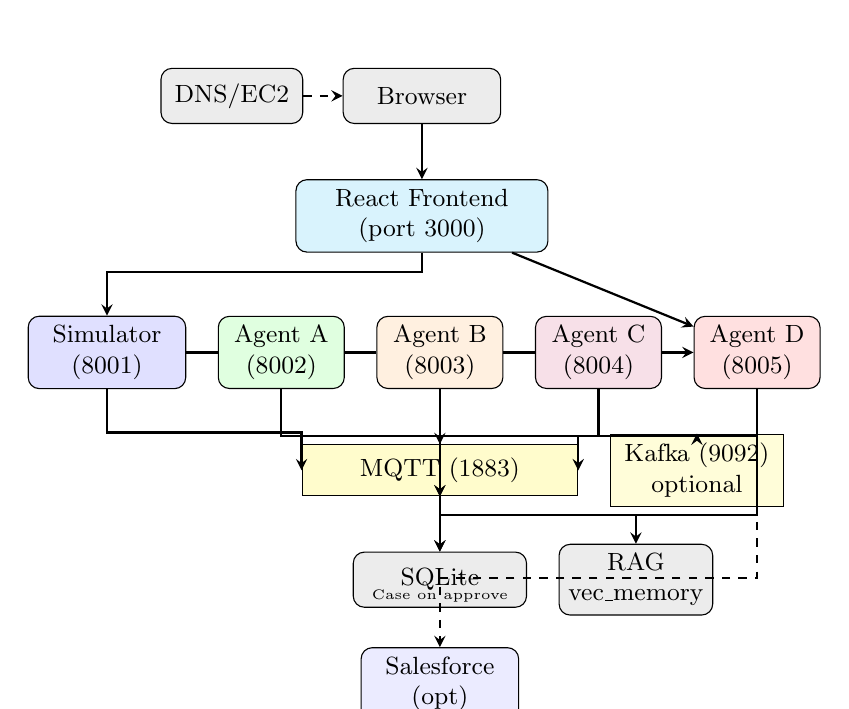
\begin{tikzpicture}[
  node distance=0.5cm,
  box/.style={rectangle, draw, rounded corners, minimum height=0.7cm, align=center, font=\small},
  bus/.style={rectangle, draw, minimum height=0.65cm, align=center, font=\small},
  arrow/.style={->, >=stealth, thick}
]
  % Layer 1: External
  \node[box, fill=gray!15, minimum width=1.8cm] (dns) {DNS/EC2};
  \node[box, fill=gray!15, right=0.5cm of dns, minimum width=2cm] (browser) {Browser};
  % Layer 2: Frontend
  \node[box, fill=cyan!15, below=0.7cm of browser, minimum width=3.2cm] (fe) {React Frontend\\(port 3000)};
  % Layer 3: Backend
  \node[box, fill=blue!12, below=0.8cm of fe, xshift=-4cm, minimum width=2cm] (sim) {Simulator\\(8001)};
  \node[box, fill=green!12, right=0.4cm of sim, minimum width=1.6cm] (a) {Agent A\\(8002)};
  \node[box, fill=orange!12, right=0.4cm of a, minimum width=1.6cm] (b) {Agent B\\(8003)};
  \node[box, fill=purple!12, right=0.4cm of b, minimum width=1.6cm] (c) {Agent C\\(8004)};
  \node[box, fill=red!12, right=0.4cm of c, minimum width=1.6cm] (d) {Agent D\\(8005)};
  % Layer 4: Message bus
  \node[bus, fill=yellow!20, below=0.7cm of b, minimum width=3.5cm] (mqtt) {MQTT (1883)};
  \node[bus, fill=yellow!15, right=0.4cm of mqtt, minimum width=2.2cm] (kafka) {Kafka (9092)\\optional};
  % Layer 5: Data
  \node[box, fill=gray!15, below=0.7cm of mqtt, minimum width=2.2cm] (db) {SQLite};
  \node[box, fill=gray!15, right=0.4cm of db, minimum width=1.8cm] (rag) {RAG\\vec\_memory};
  % Layer 6: External (optional)
  \node[box, fill=blue!8, below=0.5cm of db, minimum width=2cm] (sf) {Salesforce\\(opt)};
  % Arrows
  \draw[arrow, dashed] (dns) -- (browser);
  \draw[arrow] (browser) -- (fe);
  \draw[arrow] (fe) -- (d);
  \draw[arrow] (fe.south) -- ++(0,-0.25) -| (sim.north);
  \draw[arrow] (sim) -- (a) -- (b) -- (c) -- (d);
  \draw[arrow] (sim.south) -- ++(0,-0.55) -| (mqtt.west);
  \draw[arrow] (a.south) -- ++(0,-0.6) -| (mqtt.south);
  \draw[arrow] (b.south) -- (mqtt.north);
  \draw[arrow] (b.south) -- ++(0,-0.6) -| (kafka.north);
  \draw[arrow] (c.south) -- ++(0,-0.6) -| (mqtt.south);
  \draw[arrow] (d.south) -- ++(0,-0.6) -| (mqtt.east);
  \draw[arrow] (mqtt) -- (db);
  \draw[arrow] (d.south) -- ++(0,-1.6) -| (rag.north);
  \draw[arrow] (d.south) -- ++(0,-1.6) -| (db.north);
  \draw[arrow, dashed] (d.south) -- ++(0,-2.4) -| (sf.north) node[near end, font=\tiny, above] {Case on approve};
\end{tikzpicture}
\caption{Complete system architecture: frontend (React), backend (Simulator + Agents A--D), message buses (MQTT, optional Kafka), database (SQLite), RAG, and optional Salesforce (Case creation on approve). HTTP for API/frontend; MQTT for streaming events; Kafka for Agent B diagnosis queue.}
\label{fig:architecture_full}
\end{figure}

\section{Communication Links}

The system uses HTTP, MQTT, Kafka (optional), and outbound HTTP for external integrations. Table~\ref{tab:comm} summarizes their roles.

\begin{table}[htbp]
\centering
\caption{Communication protocols and their roles.}
\label{tab:comm}
\setlength{\tabcolsep}{6pt}
\begin{tabular}{llp{6.8cm}}
\toprule
\textbf{Protocol} & \textbf{Port} & \textbf{Description} \\
\midrule
HTTP & 8001, 8002--8005 & REST API; health checks; frontend proxy; Simulator control \\
MQTT & 1883 & Pub/sub: telemetry, alerts, diagnosis, tickets, feedback \\
Kafka & 9092 (optional) & Agent B diagnosis queue; decouples MQTT from LLM \\
HTTP (outbound) & 443 & Agent D: Salesforce REST API (Case creation on approve, optional) \\
\bottomrule
\end{tabular}
\end{table}

\textbf{HTTP:} Each backend service exposes an HTTP API (FastAPI). The frontend proxies \texttt{/api} to Agent D (8005) and \texttt{/simulator} to Simulator (8001). External access uses DNS or EC2 public IP; ports 8001 and 8005 are typically exposed for web and API access.

\textbf{MQTT:} All agents communicate via MQTT pub/sub. The Simulator publishes telemetry to \texttt{telemetry/\{asset\_id\}}; Agent A subscribes, detects anomalies, and publishes to \texttt{alerts/\{asset\_id\}}; Agent B subscribes to alerts and publishes diagnosis to \texttt{diagnosis/\{asset\_id\}}; Agent C subscribes to diagnosis and publishes tickets to \texttt{tickets/\{asset\_id\}}; Agent D publishes feedback to \texttt{feedback/\{asset\_id\}}.

\textbf{Kafka:} When configured (\texttt{KAFKA\_BOOTSTRAP\_SERVERS}), Agent B uses Kafka to queue diagnosis requests. The MQTT callback enqueues alerts to the \texttt{diagnosis-queue} topic; a consumer runs the ReAct agent asynchronously. This decouples MQTT from LLM latency and avoids blocking the alert handler.

\textbf{External HTTP:} Agent D optionally calls the Salesforce REST API when a reviewer approves a diagnosis and checks ``Create Salesforce Case.'' The Case is created with Subject (root cause), Description, and picklist fields; a ticket row is stored locally. Configuration uses \texttt{SALESFORCE\_DOMAIN} and access token or OAuth credentials.

\section{LLM, Agent, and ReAct}

The diagnosis agent uses the ReAct paradigm~\cite{yao2023react}: interleaving Thought, Action, and Observation. The LLM reasons over tool outputs and produces structured JSON with root cause, confidence, and evidence. Figure~\ref{fig:react} illustrates the ReAct loop. The agent perceives (alerts), reasons (Thought), acts (tool calls), observes (tool results), and repeats until it produces a final answer. Table~\ref{tab:agentb} lists the tools available to Agent B.

\begin{figure}[htbp]
\centering
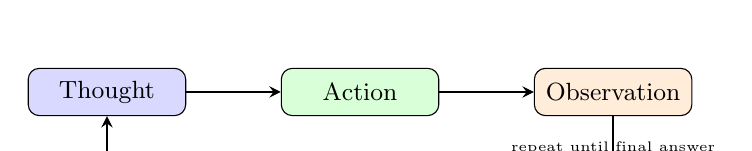
\begin{tikzpicture}[
  node distance=1.2cm,
  box/.style={rectangle, draw, rounded corners, minimum width=2cm, minimum height=0.6cm, align=center, font=\small},
  arrow/.style={->, >=stealth, thick}
]
  \node[box, fill=blue!15] (thought) {Thought};
  \node[box, fill=green!15, right=of thought] (action) {Action};
  \node[box, fill=orange!15, right=of action] (obs) {Observation};
  \draw[arrow] (thought) -- (action);
  \draw[arrow] (action) -- (obs);
  \draw[arrow] (obs.south) -- ++(0,-0.5) -| (thought.south);
  \node[below=0.2cm of obs, font=\tiny] {repeat until final answer};
\end{tikzpicture}
\caption{ReAct loop: Thought $\rightarrow$ Action $\rightarrow$ Observation. The LLM reasons, calls a tool, observes the result, and iterates.}
\label{fig:react}
\end{figure}

\begin{table}[htbp]
\centering
\caption{Agent B (Diagnosis) tools.}
\label{tab:agentb}
\begin{tabular}{ll}
\toprule
\textbf{Tool} & \textbf{Description} \\
\midrule
query\_rules & Search diagnosis rules by keywords (signal names, fault types) \\
query\_telemetry & Get recent telemetry for an asset (time range, limit) \\
query\_alerts & Get recent alerts for an asset \\
\bottomrule
\end{tabular}
\end{table}

\section{RAG Design}

RAG indexes alerts, diagnoses, rules, feedback, and chat messages into a vector store~\cite{lewis2020rag}. Agent D uses semantic search (sqlite-vec, all-MiniLM-L6-v2) for query\_similar\_diagnoses, query\_similar\_rules, and related tools~\cite{reimers2019sentence,sqlitevec2024}. Figure~\ref{fig:rag} shows the indexing and retrieval flow. Table~\ref{tab:agentd} lists the RAG and VLM tools available to Agent D.

\begin{figure}[htbp]
\centering
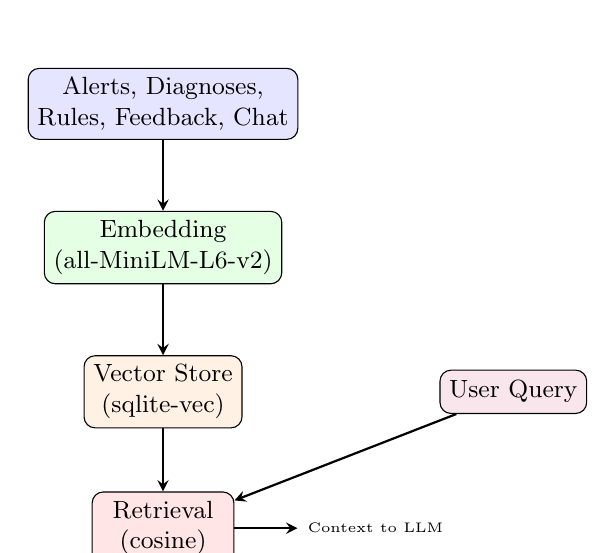
\begin{tikzpicture}[
  node distance=0.9cm,
  box/.style={rectangle, draw, rounded corners, minimum width=1.8cm, minimum height=0.55cm, align=center, font=\small},
  arrow/.style={->, >=stealth, thick}
]
  \node[box, fill=blue!10] (src) {Alerts, Diagnoses,\\Rules, Feedback, Chat};
  \node[box, fill=green!10, below=of src] (emb) {Embedding\\(all-MiniLM-L6-v2)};
  \node[box, fill=orange!10, below=of emb] (vec) {Vector Store\\(sqlite-vec)};
  \node[box, fill=purple!10, right=2.5cm of vec] (query) {User Query};
  \node[box, fill=red!10, below=0.8cm of vec] (ret) {Retrieval\\(cosine)};
  \draw[arrow] (src) -- (emb);
  \draw[arrow] (emb) -- (vec);
  \draw[arrow] (query) -- (ret);
  \draw[arrow] (vec) -- (ret);
  \draw[arrow] (ret.east) -- ++(0.8,0) node[right, font=\tiny] {Context to LLM};
\end{tikzpicture}
\caption{RAG flow: indexing (left) and retrieval (right). Documents are embedded and stored; queries retrieve similar vectors for context.}
\label{fig:rag}
\end{figure}

\begin{table}[htbp]
\centering
\caption{Agent D (Review) RAG and VLM tools.}
\label{tab:agentd}
\begin{tabular}{ll}
\toprule
\textbf{Tool} & \textbf{Description} \\
\midrule
query\_similar\_diagnoses & Semantic search for similar past diagnoses \\
query\_similar\_rules & Semantic search for relevant rules \\
query\_similar\_alerts & Semantic search for similar alerts \\
query\_similar\_feedback & Semantic search for past feedback \\
query\_similar\_chat & Semantic search for past chat \\
analyze\_image\_with\_vlm & Analyze image (e.g., 3D pump render) via VLM \\
\bottomrule
\end{tabular}
\end{table}

\section{Simulator}

The simulator models pump, piping, and bearing physics. Fault injection supports bearing\_wear, clogging, valve\_stuck, sensor\_drift, and noise\_burst. Scenarios are defined in JSON scripts. Table~\ref{tab:faults} summarizes the fault types and their physical effects.

\begin{table}[htbp]
\centering
\caption{Fault types and physical effects.}
\label{tab:faults}
\begin{tabular}{lll}
\toprule
\textbf{Fault Type} & \textbf{Physical Effect} & \textbf{Signals Affected} \\
\midrule
bearing\_wear & Increased friction, vibration & vibration\_rms, bearing\_temp\_c \\
clogging & Flow restriction, pressure rise & flow\_m3h, pressure\_bar \\
valve\_stuck & Valve position mismatch & valve\_open\_pct, flow\_m3h \\
sensor\_drift & Bias in sensor reading & temp\_c, pressure\_bar \\
noise\_burst & Transient spike & any signal \\
\bottomrule
\end{tabular}
\end{table}

\section{Agent A (Monitor)}

Agent A subscribes to telemetry, applies threshold and slope-based detection with duration checks, and publishes alerts to MQTT. A sliding-window buffer maintains recent samples for computing statistics. Threshold checks require a signal to exceed a configured limit; duration checks require the violation to persist for a minimum time before triggering an alert, reducing false positives from transient noise. Slope-based detection identifies trends (e.g., rising temperature) that may indicate gradual degradation. Figure~\ref{fig:agent_a} shows the internal structure.

\begin{figure}[htbp]
\centering
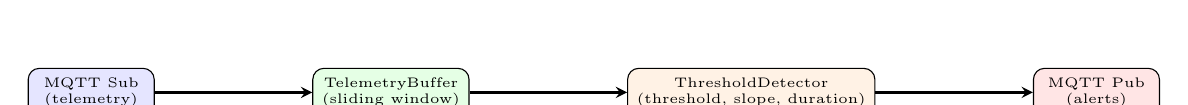
\begin{tikzpicture}[
  node distance=0.5cm,
  box/.style={rectangle, draw, rounded corners, minimum width=1.6cm, minimum height=0.5cm, align=center, font=\tiny},
  arrow/.style={->, >=stealth, thick}
]
  \node[box, fill=blue!10] (mqtt) {MQTT Sub\\(telemetry)};
  \node[box, fill=green!10, right=2cm of mqtt] (buf) {TelemetryBuffer\\(sliding window)};
  \node[box, fill=orange!10, right=2cm of buf] (det) {ThresholdDetector\\(threshold, slope, duration)};
  \node[box, fill=red!10, right=2cm of det] (pub) {MQTT Pub\\(alerts)};
  \draw[arrow] (mqtt) -- (buf);
  \draw[arrow] (buf) -- (det);
  \draw[arrow] (det) -- (pub);
\end{tikzpicture}
\caption{Agent A (Monitor) architecture: MQTT subscription $\rightarrow$ TelemetryBuffer $\rightarrow$ ThresholdDetector $\rightarrow$ MQTT publish.}
\label{fig:agent_a}
\end{figure}

\section{Agent B (Diagnosis)}

Agent B subscribes to alerts, runs a ReAct agent with tools (Table~\ref{tab:agentb}), retrieves rules from Markdown documents, and publishes diagnosis reports. The diagnosis report schema includes root\_cause, confidence, impact, recommended\_actions, and evidence. The agent parses the LLM's final JSON output and publishes to the diagnosis topic. When Kafka is enabled, alerts are queued and a consumer runs diagnosis asynchronously. Figure~\ref{fig:agent_b} shows the architecture.

\begin{figure}[htbp]
\centering
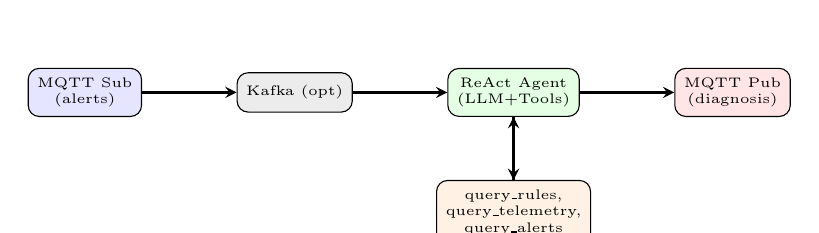
\begin{tikzpicture}[
  node distance=0.45cm,
  box/.style={rectangle, draw, rounded corners, minimum width=1.4cm, minimum height=0.5cm, align=center, font=\tiny},
  arrow/.style={->, >=stealth, thick}
]
  \node[box, fill=blue!10] (mqtt) {MQTT Sub\\(alerts)};
  \node[box, fill=gray!15, right=1.2cm of mqtt, minimum width=1.2cm] (kafka) {Kafka (opt)};
  \node[box, fill=green!10, right=1.2cm of kafka] (react) {ReAct Agent\\(LLM+Tools)};
  \node[box, fill=orange!10, below=0.8cm of react] (tools) {query\_rules,\\query\_telemetry,\\query\_alerts};
  \node[box, fill=red!10, right=1.2cm of react] (pub) {MQTT Pub\\(diagnosis)};
  \draw[arrow] (mqtt) -- (kafka);
  \draw[arrow] (kafka) -- (react);
  \draw[arrow] (react) -- (tools);
  \draw[arrow] (tools) -- (react);
  \draw[arrow] (react) -- (pub);
\end{tikzpicture}
\caption{Agent B (Diagnosis) architecture: MQTT $\rightarrow$ Kafka (optional) $\rightarrow$ ReAct agent with tools $\rightarrow$ MQTT publish.}
\label{fig:agent_b}
\end{figure}

\section{Agent C (Ticket)}

Agent C creates review requests from diagnoses. No LLM is used; it is a rule-based relay. For each diagnosis, it creates a review\_request with status=``pending'' and queues it for Agent D approval.

\section{Agent D (Review)}

Agent D provides a human-in-the-loop interface with RAG tools (Table~\ref{tab:agentd}), approve/reject workflow, and optional external integrations. When a reviewer approves a diagnosis, they may optionally create a Salesforce Case via REST API; the Case form is pre-filled with Subject (root cause), Description (diagnosis summary), Priority, Status, and other picklist fields fetched from the Salesforce org. Configuration uses \texttt{SALESFORCE\_DOMAIN} and either \texttt{SALESFORCE\_ACCESS\_TOKEN} or OAuth (client\_id, client\_secret, username, password). If not configured, approval is recorded locally only. The frontend is a React web app with pages for Review Queue, Alerts, Sensors, Chat, and Scenarios. The Chat page streams ReAct steps via Server-Sent Events (SSE). The agent can call analyze\_image\_with\_vlm to analyze 3D pump renderings or dashboard screenshots~\cite{li2022blip,liu2023llava}. Figure~\ref{fig:agent_d} shows the architecture.

\begin{figure}[htbp]
\centering
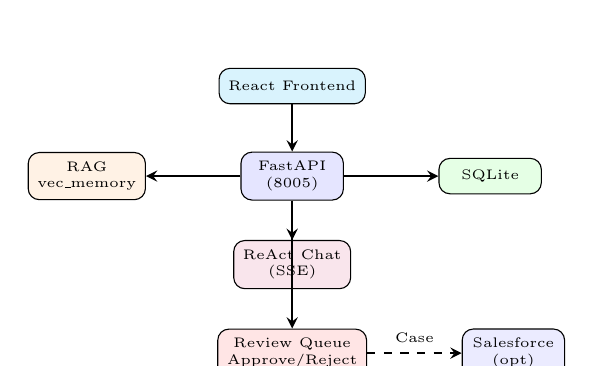
\begin{tikzpicture}[
  node distance=0.4cm,
  box/.style={rectangle, draw, rounded corners, minimum width=1.3cm, minimum height=0.45cm, align=center, font=\tiny},
  arrow/.style={->, >=stealth, thick}
]
  \node[box, fill=cyan!15] (fe) {React Frontend};
  \node[box, fill=blue!10, below=0.6cm of fe] (api) {FastAPI\\(8005)};
  \node[box, fill=green!10, right=1.2cm of api] (db) {SQLite};
  \node[box, fill=orange!10, left=1.2cm of api] (rag) {RAG\\vec\_memory};
  \node[box, fill=purple!10, below=0.5cm of api] (chat) {ReAct Chat\\(SSE)};
  \node[box, fill=red!10, below=0.5cm of chat] (review) {Review Queue\\Approve/Reject};
  \node[box, fill=blue!8, right=1.2cm of review] (sf) {Salesforce\\(opt)};
  \draw[arrow] (fe) -- (api);
  \draw[arrow] (api) -- (db);
  \draw[arrow] (api) -- (rag);
  \draw[arrow] (api) -- (chat);
  \draw[arrow] (api) -- (review);
  \draw[arrow, dashed] (review) -- (sf) node[midway, above, font=\tiny] {Case};
\end{tikzpicture}
\caption{Agent D (Review) architecture: React frontend $\rightarrow$ FastAPI; API uses SQLite, RAG, ReAct chat (SSE), review queue, and optional Salesforce Case creation on approve.}
\label{fig:agent_d}
\end{figure}

\subsection{Salesforce OAuth and Case Architecture}

When Salesforce integration is enabled, Agent D authenticates via OAuth 2.0~\cite{ietf2012oauth2} and creates Cases through the REST API~\cite{salesforce2024rest}. This subsection describes the OAuth connection flow and the Case object architecture.

\textbf{OAuth Connection.} The system supports two configuration methods. \textit{Method A (Access Token):} Provide \texttt{SALESFORCE\_DOMAIN} and a pre-obtained \texttt{SALESFORCE\_ACCESS\_TOKEN}; the token is obtained manually (e.g., via curl) using the password grant. \textit{Method B (Password Flow):} Provide \texttt{SALESFORCE\_DOMAIN}, \texttt{SALESFORCE\_CLIENT\_ID}, \texttt{SALESFORCE\_CLIENT\_SECRET}, \texttt{SALESFORCE\_USERNAME}, and \texttt{SALESFORCE\_PASSWORD} (login password concatenated with the user's Security Token). The connector requests an access token from \texttt{https://\{domain\}/services/oauth2/token} with \texttt{grant\_type=password}. A Connected App must be created in Salesforce Setup (App Manager) with OAuth enabled; required scopes include \texttt{api} and \texttt{refresh\_token}. Optionally, client credentials flow is supported if the Connected App is configured for it. Figure~\ref{fig:salesforce_oauth} illustrates the OAuth and Case creation flow.

\begin{figure}[htbp]
\centering
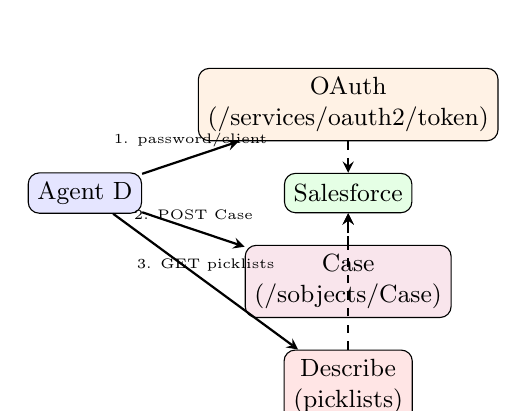
\begin{tikzpicture}[
  node distance=0.6cm,
  box/.style={rectangle, draw, rounded corners, minimum height=0.5cm, align=center, font=\small},
  arrow/.style={->, >=stealth, thick}
]
  \node[box, fill=blue!10] (agentd) {Agent D};
  \node[box, fill=green!10, right=1.8cm of agentd] (sf) {Salesforce};
  \node[box, fill=orange!10, above=0.4cm of sf] (oauth) {OAuth\\(/services/oauth2/token)};
  \node[box, fill=purple!10, below=0.4cm of sf] (case) {Case\\(/sobjects/Case)};
  \node[box, fill=red!10, below=0.4cm of case] (desc) {Describe\\(picklists)};
  \draw[arrow] (agentd) -- (oauth) node[midway, above, font=\tiny] {1. password/client};
  \draw[arrow] (agentd) -- (case) node[midway, above, font=\tiny] {2. POST Case};
  \draw[arrow] (agentd) -- (desc) node[midway, above, font=\tiny] {3. GET picklists};
  \draw[arrow, dashed] (oauth) -- (sf);
  \draw[arrow, dashed] (case) -- (sf);
  \draw[arrow, dashed] (desc) -- (sf);
\end{tikzpicture}
\caption{Salesforce OAuth and Case flow: (1) Agent D obtains access token via password or client credentials flow; (2) creates Case via REST POST on approve; (3) fetches Case picklists via Describe API for form prefill.}
\label{fig:salesforce_oauth}
\end{figure}

\textbf{Case Object Architecture.} Case is a standard Salesforce object for customer support~\cite{salesforce2024rest}. The connector sends a POST to \texttt{/services/data/v58.0/sobjects/Case} with JSON payload: \texttt{Subject} (root cause, prefixed with \texttt{[asset\_id]}), \texttt{Description} (diagnosis summary), \texttt{Status}, \texttt{Priority}, \texttt{Origin}, \texttt{Type}, and \texttt{Reason}. Status, Priority, Origin, Type, and Reason are picklist fields; valid values are fetched from \texttt{/sobjects/Case/describe} so the frontend can render dropdowns. On success, the API returns the Case Id; Agent D stores a ticket row locally with \texttt{ticket\_id} and \texttt{url} (Lightning record URL). The \texttt{TicketConnector} interface allows swapping Salesforce for other CRM systems (e.g., ServiceNow, Zendesk) with minimal changes.

\section{Message Bus and Data Schemas}

MQTT topics follow the convention in Table~\ref{tab:mqtt}. Telemetry, AlertEvent, DiagnosisReport, Ticket, and Feedback schemas define the message payloads. Table~\ref{tab:schemas} summarizes the key fields for each payload type. Each agent publishes to downstream topics and subscribes to upstream topics.

\begin{table}[htbp]
\centering
\caption{Message payload schemas (key fields).}
\label{tab:schemas}
\small
\begin{tabular}{llp{6.5cm}}
\toprule
\textbf{Schema} & \textbf{Source} & \textbf{Key Fields} \\
\midrule
Telemetry & Simulator & ts, plant\_id, asset\_id, signals (pressure\_bar, flow\_m3h, temp\_c, bearing\_temp\_c, vibration\_rms, rpm, motor\_current\_a, valve\_open\_pct), truth (fault, severity) \\
\addlinespace
AlertEvent & Agent A & ts, plant\_id, asset\_id, severity (warning/critical), alerts (signal, score, method, evidence) \\
\addlinespace
DiagnosisReport & Agent B & ts, plant\_id, asset\_id, root\_cause, confidence, impact, recommended\_actions, evidence \\
\addlinespace
Ticket & Agent C & ts, plant\_id, asset\_id, ticket\_system, ticket\_id, url \\
\addlinespace
Feedback & Agent D & ts, plant\_id, asset\_id, ticket\_id, review\_decision (approved/rejected/edited), final\_root\_cause, notes \\
\bottomrule
\end{tabular}
\end{table}

\begin{table}[htbp]
\centering
\caption{MQTT topic convention.}
\label{tab:mqtt}
\begin{tabular}{ll}
\toprule
\textbf{Topic} & \textbf{Description} \\
\midrule
telemetry/\{asset\_id\} & Raw telemetry from Simulator \\
alerts/\{asset\_id\} & Alerts from Agent A \\
diagnosis/\{asset\_id\} & Diagnosis reports from Agent B \\
tickets/\{asset\_id\} & Tickets from Agent C \\
feedback/\{asset\_id\} & Human feedback from Agent D \\
vision/\{asset\_id\} & Vision image paths (optional) \\
\bottomrule
\end{tabular}
\end{table}

\section{Database Design}

SQLite stores telemetry, alerts, diagnosis, vision images, tickets, review requests, chat sessions, chat messages, chat steps, and feedback. Table~\ref{tab:db} summarizes the main tables. The vec\_memory virtual table (sqlite-vec) stores 384-dimensional embeddings for RAG; it is indexed by cosine similarity.

\begin{table}[htbp]
\centering
\caption{Database tables.}
\label{tab:db}
\begin{tabular}{ll}
\toprule
\textbf{Table} & \textbf{Description} \\
\midrule
telemetry & Sensor readings from Simulator \\
alerts & Alerts from Agent A \\
diagnosis & Diagnosis reports from Agent B \\
vision\_images & Image paths from Simulator \\
vision\_analysis & VLM analysis results \\
tickets & Tickets from Agent C \\
review\_requests & Pending review queue \\
chat\_sessions, chat\_messages, chat\_steps & Chat persistence \\
feedback & Human approval/rejection \\
vec\_memory & Vector embeddings (RAG) \\
\bottomrule
\end{tabular}
\end{table}

\section{Frontend Design}

The Agent D frontend is a React single-page application with the following pages: Review Queue (pending diagnoses, approve/reject), Alerts (alert list with filtering), Sensors (real-time telemetry display), Chat (ReAct agent with SSE streaming), and Scenarios (simulator control). The frontend communicates with the Agent D backend via REST API and SSE for chat streaming. The layout uses a sidebar for navigation and a main content area that switches based on route.

% ========== Chapter 4: Implementation ==========
\chapter{Implementation}
\label{ch:impl}

This chapter describes the implementation of the multi-agent powerplant monitoring system. Each component is built with Python 3.11 and integrates via MQTT and REST APIs. The implementation follows the architecture described in Chapter~\ref{ch:design}.

\section{Technology Stack}

The system uses a cohesive technology stack chosen for rapid development, interoperability, and reproducibility. The backend is implemented in Python; the Agent D frontend is a React single-page application. Table~\ref{tab:tech} summarizes the main components by category.

\begin{table}[htbp]
\centering
\caption{Technology stack by category.}
\label{tab:tech}
\begin{tabular}{ll}
\toprule
\textbf{Category} & \textbf{Technologies} \\
\midrule
Runtime & Python 3.11 \\
Web framework & FastAPI, pydantic, pydantic-settings, uvicorn \\
Message bus & MQTT (paho-mqtt), Mosquitto broker; Kafka (kafka-python, optional) \\
Agent framework & LangChain, LangGraph, langchain-openai \\
RAG / vector search & sqlite-vec, sentence-transformers \\
Streaming & sse-starlette (Server-Sent Events) \\
HTTP client & httpx \\
Frontend & React 18, Vite, React Router, Axios, Recharts, react-markdown \\
Evaluation & matplotlib \\
Optional / external & Salesforce (OAuth, Case API), GitHub API, pyvista (3D), anthropic (Claude Vision) \\
\bottomrule
\end{tabular}
\end{table}

\subsection{Backend Stack}

Python 3.11 provides modern type hints and performance improvements. FastAPI~\cite{fastapi2024} offers async support, automatic OpenAPI documentation, and Pydantic validation for request/response schemas. Configuration is managed via \texttt{pydantic-settings} with environment variables and an optional \texttt{.env} file. MQTT via paho-mqtt~\cite{oasis2019mqtt} enables lightweight pub/sub for telemetry and alerts; Kafka (kafka-python) is optionally used as a diagnosis queue for Agent B when high throughput is needed. LangChain~\cite{langchain2024} and LangGraph~\cite{langgraph2024} implement the ReAct agent loop~\cite{yao2023react} with tool calling; \texttt{langchain-openai} provides the LLM interface (compatible with DeepSeek and OpenAI). The RAG pipeline uses sqlite-vec~\cite{sqlitevec2024} for in-process vector storage and sentence-transformers~\cite{reimers2019sentence,reimers2024sentence} (all-MiniLM-L6-v2) for embeddings, avoiding external API calls. Agent D streams chat responses via sse-starlette; httpx is used for outbound HTTP requests. Matplotlib generates evaluation charts for detection rates and diagnosis accuracy.

\subsection{Optional Components}

Several optional components extend the system when configured. \textbf{Salesforce:} Agent D uses the Salesforce REST API~\cite{salesforce2024rest} with OAuth 2.0~\cite{ietf2012oauth2} (password flow or access token) to create Cases when a reviewer approves a diagnosis; the \texttt{SalesforceConnector} in \texttt{shared\_lib/integrations/salesforce.py} implements the \texttt{TicketConnector} interface. \textbf{GitHub:} Agent C can create GitHub Issues as tickets when \texttt{GITHUB\_TOKEN} and \texttt{GITHUB\_REPO} are set. \textbf{pyvista:} The simulator optionally renders 3D pump visualizations for the vision pipeline. \textbf{anthropic:} Claude Vision (Claude 3) is used for \texttt{analyze\_image\_with\_vlm} when multimodal analysis is enabled~\cite{li2022blip,liu2023llava}; the VLM analyzes 3D renderings or dashboard screenshots. All optional components are configured via environment variables and degrade gracefully when not present.

\subsection{Frontend Stack}

The Agent D review dashboard is a React 18 single-page application built with Vite. React Router DOM handles client-side routing (Review Queue, Alerts, Sensors, Chat, Scenarios). Axios performs REST API calls to the Agent D backend. Recharts renders real-time telemetry charts on the Sensors page. React Markdown with remark-gfm displays chat responses and ReAct reasoning steps with proper markdown formatting (tables, code blocks). The frontend is served as static assets by the Agent D FastAPI server after \texttt{npm run build}; in development, Vite provides hot module replacement. The build output targets modern browsers (browserslist: \texttt{>0.2\%, not dead}).

\subsection{Project Structure and Configuration}

The project is organized as a monorepo: \texttt{simulator-service/} (simulator), \texttt{agent-monitor/}, \texttt{agent-diagnosis/}, \texttt{agent-ticket/}, \texttt{agent-review/} (backend and frontend), \texttt{shared\_lib/} (models, config, db, embeddings, vector\_db, vector\_indexing), \texttt{scripts/} (init\_db, start\_backend\_ec2), and \texttt{evaluation/}. Each service runs as a separate process; they share \texttt{shared\_lib} and communicate via MQTT and REST. Optional integrations (GitHub for Agent C tickets, Salesforce for Case creation on approval) are configured via environment variables when needed.

\section{Simulator Implementation}

The simulator produces realistic pump telemetry with configurable faults. It consists of four physical models (pump, pipe, bearing, motor), a fault injector, and a scenario executor that drives the simulation loop from JSON definitions. The models are based on first-principles physics~\cite{reeh2023physical}; faults modify model parameters or outputs to produce detectable anomalies.

\subsection{Physical Models}

Each model implements equations from fluid mechanics, electrical engineering, or mechanical vibration. The models are coupled: the pump and pipe determine the operating point $(Q, H)$; the pump power drives the motor current and bearing load; the bearing yields vibration and temperature.

\subsubsection{Pump Model}

The \texttt{PumpModel} uses a quadratic head-flow curve and affinity laws~\cite{reeh2023physical}. At rated conditions $(n_N, Q_N, H_N)$, the pump head is
\begin{equation}
H_{\text{pump}}(Q, n) = H_{\text{shutoff}}(n) - a \cdot Q^2, \quad H_{\text{shutoff}}(n) = H_{\text{shutoff},N} \cdot (n/n_N)^2,
\end{equation}
where $n$ is rpm, $Q$ is flow (m$^3$/h), and $a = (H_{\text{shutoff},N} - H_N) / Q_N^2$. Affinity laws scale flow and head with speed: $Q \propto n$, $H \propto n^2$. Valve opening limits maximum flow: $Q_{\max} = Q_N \cdot (n/n_N) \cdot (\text{valve}/100)$. Efficiency is parabolic around the best-efficiency point:
\begin{equation}
\eta(Q) = \eta_N \cdot \left(1 - \left(\frac{Q - Q_{\text{opt}}}{Q_{\text{opt}}}\right)^2\right), \quad Q_{\text{opt}} = Q_N \cdot (n/n_N).
\end{equation}
Shaft power follows $P_{\text{shaft}} = \rho g Q H / \eta$ (with $\rho = 1000$\,kg/m$^3$, $g = 9.81$\,m/s$^2$). The operating point is found by solving $H_{\text{pump}}(Q) = H_{\text{system}}(Q)$ via binary search. Listing~\ref{lst:pump_head} shows \texttt{compute\_head} and \texttt{solve\_operating\_point}.

\begin{lstlisting}[language=Python, caption={PumpModel.compute\_head and solve\_operating\_point (simulator-service/models/pump\_model.py)}, label=lst:pump_head]
def compute_head(self, Q: float, rpm: float) -> float:
    n_ratio = rpm / self.n_N
    H_shutoff_scaled = self.H_shutoff * (n_ratio ** 2)
    H = H_shutoff_scaled - self.a_coeff * (Q ** 2)
    return max(0.0, H)

def solve_operating_point(self, rpm, valve_open_pct, system_head_func):
    _, Q_max = self.compute_head_flow_curve(rpm, valve_open_pct)
    Q_low, Q_high = 0.0, Q_max
    for _ in range(50):
        Q_mid = (Q_low + Q_high) / 2.0
        H_pump = self.compute_head(Q_mid, rpm)
        H_system = system_head_func(Q_mid)
        if abs(H_pump - H_system) < 0.01:
            return Q_mid, H_pump
        if H_pump > H_system: Q_low = Q_mid
        else: Q_high = Q_mid
    Q_final = (Q_low + Q_high) / 2.0
    return Q_final, self.compute_head(Q_final, rpm)
\end{lstlisting}

\subsubsection{Pipe System Model}

The \texttt{PipeSystemModel} uses the Darcy-Weisbach equation~\cite{white2016fluid} for friction loss. System head is
\begin{equation}
H_{\text{system}}(Q) = R \cdot Q_{\text{m}^3/\text{s}}^2 + H_{\text{static}},
\end{equation}
where $R = f(L/D)/(2gA^2) + K/(2gA^2)$ combines pipe friction ($f \approx 0.02$) and fittings loss ($K$). Flow is converted from m$^3$/h to m$^3$/s for the quadratic term. Clogging increases resistance: $R_{\text{current}} = R_{\text{base}} \cdot \text{clogging\_factor}$. Listing~\ref{lst:pipe} shows the implementation.

\begin{lstlisting}[language=Python, caption={PipeSystemModel.compute\_system\_head and set\_clogging\_resistance}, label=lst:pipe]
def compute_system_head(self, Q: float) -> float:
    Q_m3s = Q / 3600.0
    H_dynamic = self.R_current * (Q_m3s ** 2)
    return H_dynamic + self.H_static

def set_clogging_resistance(self, clogging_factor: float):
    self.clogging_factor = max(1.0, clogging_factor)
    self.R_current = self.R_base * self.clogging_factor
\end{lstlisting}

\subsubsection{Bearing Model}

The \texttt{BearingModel} tracks wear level $d \in [0, 1]$ (0 = healthy, 1 = failure), following vibration-based condition monitoring principles~\cite{randall2011vibration}. Wear accumulates linearly: $d \leftarrow d + \dot{d} \cdot \Delta t$. Vibration RMS (mm/s) increases non-linearly with wear:
\begin{equation}
v = v_{\text{base}} \cdot (1 + 2d + 5d^3) \cdot (1 + 0.2(\lambda - 1)),
\end{equation}
where $\lambda$ is load factor ($P_{\text{shaft}}/10$ kW). Temperature rises with heat generation (increased friction) and degraded thermal dissipation:
\begin{equation}
\Delta T = \text{heat\_gen} \cdot \text{thermal\_resistance} \cdot 20, \quad \text{heat\_gen} = \lambda(1 + 3d), \quad \text{thermal\_resistance} = \frac{0.5}{1 + 0.5d}.
\end{equation}
Listing~\ref{lst:bearing_model} shows \texttt{compute\_vibration} and \texttt{compute\_bearing\_temperature}.

\begin{lstlisting}[language=Python, caption={BearingModel.compute\_vibration and compute\_bearing\_temperature}, label=lst:bearing_model]
def compute_vibration(self, load_factor: float = 1.0) -> float:
    wear_effect = 1.0 + self.wear_level * 2.0 + (self.wear_level ** 3) * 5.0
    load_effect = 1.0 + 0.2 * (load_factor - 1.0)
    return max(0.1, self.base_vibration_rms * wear_effect * load_effect)

def compute_bearing_temperature(self, load_factor: float = 1.0) -> float:
    heat_generation_factor = load_factor * (1.0 + self.wear_level * 3.0)
    thermal_resistance = 0.5 / (1.0 + self.wear_level * 0.5)
    temp_rise = heat_generation_factor * thermal_resistance * 20.0
    base_temp_rise = self.base_bearing_temp - self.ambient_temp
    return max(self.ambient_temp, self.ambient_temp + base_temp_rise + temp_rise)
\end{lstlisting}

\subsubsection{Motor Model}

The \texttt{MotorModel} converts shaft power to motor current. Electrical power is $P_{\text{elec}} = P_{\text{shaft}} / \eta_{\text{motor}}$. For three-phase AC:
\begin{equation}
I = \frac{P_{\text{elec}}}{\sqrt{3} \cdot U \cdot \cos\phi} + I_{\text{no-load}}.
\end{equation}
Default parameters: $U = 400$\,V, $\eta_{\text{motor}} = 0.92$, $\cos\phi = 0.85$, $I_{\text{no-load}} = 5$\,A.

\subsection{Model Execution Logic}

The \texttt{ScenarioExecutor.step(dt)} runs each time step in order: (1) update setpoints (rpm, valve from scenario); (2) \texttt{fault\_injector.update\_faults} (e.g., bearing wear, clogging); (3) apply valve faults (valve\_stuck); (4) solve $H_{\text{pump}}(Q) = H_{\text{system}}(Q)$ for $(Q, H)$; (5) compute $\eta$, $P_{\text{shaft}}$, $I_{\text{motor}}$; (6) compute bearing vibration and temperature; (7) map to sensor signals (pressure $\approx 0.1 \cdot H$ bar, flow, temp, etc.); (8) apply sensor faults (drift, override, noise\_burst); (9) add Gaussian sensor noise; (10) return \texttt{Telemetry}. Listing~\ref{lst:step} shows the core loop.

\begin{lstlisting}[language=Python, caption={ScenarioExecutor.step core logic (simulator-service/scenarios/scenario\_executor.py)}, label=lst:step]
def step(self, dt: float) -> Optional[Telemetry]:
    self._update_setpoints()
    self.fault_injector.update_faults(self.current_time, dt)
    valve_actual = self.fault_injector.apply_valve_faults(self.valve_open_pct)
    Q, H = self.pump.solve_operating_point(
        self.rpm, valve_actual, self.pipe.compute_system_head
    )
    eta = self.pump.compute_efficiency(Q, self.rpm)
    P_shaft = self.pump.compute_power(Q, H, eta)
    I_motor = self.motor.compute_current(P_shaft)
    load_factor = P_shaft / 10.0
    vibration_rms = self.bearing.compute_vibration(load_factor)
    bearing_temp = self.bearing.compute_bearing_temperature(load_factor)
    true_signals = {"pressure_bar": H*0.1, "flow_m3h": Q, ...}
    sensor_signals = self.fault_injector.apply_sensor_faults(true_signals)
    self._add_sensor_noise(sensor_signals)
    self.current_time += dt
    return Telemetry(signals=..., truth=...)
\end{lstlisting}

\subsection{Fault Injector}

The \texttt{FaultInjector} maintains a mapping from fault type names to fault classes and applies fault-specific updates each time step. Listing~\ref{lst:inject} shows the \texttt{inject\_fault} method.

\begin{lstlisting}[language=Python, caption={FaultInjector.inject\_fault (simulator-service/faults/fault\_injector.py)}, label=lst:inject]
def inject_fault(self, fault_type: str, start_time: float, params: Dict[str, Any]):
    fault_map = {
        "bearing_wear": BearingWearFault,
        "clogging": CloggingFault,
        "valve_stuck": ValveStuckFault,
        "sensor_drift": SensorDriftFault,
        "sensor_stuck": SensorStuckFault,
        "sensor_override": SensorOverrideFault,
        "noise_burst": NoiseBurstFault,
    }
    fault_class = fault_map.get(fault_type)
    if fault_class:
        fault = fault_class(start_time, params)
        self.active_faults.append(fault)
    else:
        raise ValueError(f"Unknown fault type: {fault_type}")
\end{lstlisting}

Each fault type implements \texttt{update(current\_time, dt, models)} to modify physical models. For example, \texttt{BearingWearFault} increases bearing wear over time, which raises vibration and temperature (Listing~\ref{lst:bearing}).

\begin{lstlisting}[language=Python, caption={BearingWearFault.update (simulator-service/faults/fault\_types.py)}, label=lst:bearing]
def update(self, current_time: float, dt: float, models: Dict[str, Any]):
    if current_time >= self.start_time:
        self.active = True
        self.elapsed_time += dt
        bearing_model = models.get("bearing")
        if bearing_model:
            bearing_model.update_wear(self.rate_per_sec, dt)
\end{lstlisting}

\subsection{Scenario Executor}

The \texttt{ScenarioExecutor} is initialized with a scenario dictionary (from JSON) and pump config. It creates \texttt{PumpModel}, \texttt{PipeSystemModel}, \texttt{BearingModel}, and \texttt{MotorModel} from config; registers them with the fault injector; and injects faults from \texttt{scenario["faults"]}. A scenario JSON includes \texttt{name}, \texttt{duration\_sec}, \texttt{initial\_conditions} (rpm, valve\_open\_pct), \texttt{faults} (type, start\_time\_sec, params), \texttt{setpoints} (time-ordered rpm/valve changes), and optional \texttt{seed} for reproducible sensor noise. The main simulation loop (in \texttt{simulator-service/main.py}) runs \texttt{step(dt)} at \texttt{simulator\_frequency\_hz} (default 1\,Hz), publishes telemetry to MQTT, and optionally writes to the database.

\section{Agent A Implementation}

Agent A subscribes to MQTT telemetry, detects anomalies via thresholds and slopes~\cite{chandola2009anomaly,li2021intelligent}, and publishes alerts. The data flow is: MQTT callback \texttt{on\_telemetry} receives telemetry $\rightarrow$ \texttt{buffer.push(telemetry)} $\rightarrow$ \texttt{detector.detect(telemetry, buffer)} $\rightarrow$ if alert and not in cooldown: insert to DB, \texttt{index\_alert} for RAG, publish to MQTT. Two core components are \texttt{TelemetryBuffer} and \texttt{ThresholdDetector}.

\subsection{TelemetryBuffer}

\texttt{TelemetryBuffer} maintains a per-asset sliding window of recent telemetry (default \texttt{window\_sec}=120\,s, \texttt{max\_points\_per\_asset}=200). On each \texttt{push}, it appends a \texttt{BufferedPoint} and trims points older than \texttt{window\_sec}. \texttt{compute\_stats(asset\_id, signal, window\_sec)} returns mean $\mu$, std $\sigma$, and slope:
\begin{equation}
\mu = \frac{1}{n}\sum_{i=1}^n v_i, \quad \sigma = \sqrt{\frac{1}{n}\sum_{i=1}^n (v_i - \mu)^2}, \quad \text{slope} = \frac{v_n - v_1}{t_n - t_1} \quad \text{(units/sec)}.
\end{equation}
\texttt{duration\_above\_threshold(asset\_id, signal, threshold, side, window\_sec)} returns the seconds the signal has been above (side=``high'') or below (side=``low'') the threshold within the window; a single matching point is counted as 0.5\,s to allow fast triggers. Listing~\ref{lst:buffer} shows \texttt{compute\_stats} and \texttt{duration\_above\_threshold}.

\begin{lstlisting}[language=Python, caption={TelemetryBuffer.compute\_stats and duration\_above\_threshold}, label=lst:buffer]
def compute_stats(self, asset_id, signal, window_sec=None) -> Dict[str, Any]:
    points = self.get_window(asset_id, signal, window_sec)
    if len(points) < 2:
        return {"mean": None, "std": None, "slope": None}
    values = [v for _, v in points]
    mean = sum(values) / len(values)
    std = (sum((x - mean)**2 for x in values) / len(values)) ** 0.5
    dt = points[-1][0].timestamp() - points[0][0].timestamp()
    slope = (values[-1] - values[0]) / dt if dt > 0 else 0.0
    return {"mean": mean, "std": std, "slope": slope}

def duration_above_threshold(self, asset_id, signal, threshold, side="high", window_sec=None) -> float:
    points = self.get_window(asset_id, signal, window_sec)
    total_sec, n_matching = 0.0, 0
    for i in range(len(points)):
        t, v = points[i]
        above = (side == "high" and v >= threshold) or (side == "low" and v <= threshold)
        if above:
            n_matching += 1
            if i + 1 < len(points):
                total_sec += (points[i+1][0] - t).total_seconds()
    if n_matching >= 1 and total_sec < 0.5:
        total_sec = 0.5
    return total_sec
\end{lstlisting}

\subsection{ThresholdDetector}

\texttt{ThresholdDetector} checks signals against \texttt{DEFAULT\_THRESHOLDS} (Listing~\ref{lst:thresh}), implementing statistical threshold-based detection~\cite{chandola2009anomaly}. Threshold types: \textbf{low-side} (e.g., \texttt{flow\_m3h}: warning\_low, critical\_low); \textbf{high-side} (e.g., \texttt{vibration\_rms}, \texttt{bearing\_temp\_c}: warning, critical); \textbf{range} (e.g., \texttt{rpm}: min, max). Critical severity takes precedence over warning. Each \texttt{AlertDetail} includes \texttt{signal}, \texttt{score}, \texttt{method} (threshold/slope/combination), and \texttt{evidence} (value, threshold, duration, mean, std, slope). Signals in \texttt{FAST\_DURATION\_SIGNALS} (\texttt{temp\_c}, \texttt{rpm}, \texttt{valve\_flow\_mismatch}) use \texttt{min\_dur}=0.5\,s; others use \texttt{monitor\_min\_duration\_sec} (default 5\,s) to reduce false positives.

\begin{lstlisting}[language=Python, caption={DEFAULT\_THRESHOLDS (agent-monitor/detection/threshold\_detector.py)}, label=lst:thresh]
DEFAULT_THRESHOLDS = {
    "vibration_rms": {"warning": 2.8, "critical": 18.0},
    "bearing_temp_c": {"warning": 55.0, "critical": 85.0},
    "pressure_bar": {"warning_high": 7.5, "critical_high": 25.0},
    "motor_current_a": {"warning_high": 34.0, "critical_high": 45.0},
    "flow_m3h": {"warning_low": 48.0, "critical_low": 45.0},
    "rpm": {"min": 2650.0, "max": 3150.0},
}
\end{lstlisting}

Table~\ref{tab:slope} lists \texttt{DEFAULT\_SLOPE\_THRESHOLDS} for trend-based alerts. Slope is in units per second; \texttt{side}=``low'' means alert when slope falls below the threshold (e.g., flow dropping).

\begin{table}[htbp]
\centering
\caption{Slope thresholds for trend-based alerts.}
\label{tab:slope}
\small
\begin{tabular}{llll}
\toprule
\textbf{Signal} & \textbf{Warning} & \textbf{Critical} & \textbf{Side} \\
\midrule
vibration\_rms & 0.008 & 0.08 & high \\
bearing\_temp\_c & 0.38 & 0.6 & high \\
flow\_m3h & $-$0.85 & $-$5.0 & low \\
pressure\_bar & 0.25 & 1.0 & high \\
motor\_current\_a & 0.95 & 1.5 & high \\
\bottomrule
\end{tabular}
\end{table}

When a buffer is provided, the detector only emits a threshold alert if the signal has sustained the breach for at least \texttt{min\_dur} seconds (Listing~\ref{lst:duration}).

\begin{lstlisting}[language=Python, caption={Duration check in ThresholdDetector.detect}, label=lst:duration]
min_dur = 0.5 if signal_name in FAST_DURATION_SIGNALS else self.min_duration_sec
if buffer and min_dur > 0:
    thr_val = rule.get("critical") or rule.get("critical_high") or rule.get("critical_low")
    if thr_val is not None:
        dur = buffer.duration_above_threshold(
            telemetry.asset_id, signal_name, thr_val, side, self.window_sec
        )
        if dur < min_dur:
            continue  # Not sustained long enough
\end{lstlisting}

\textbf{Valve-flow mismatch} is a composite rule: valve $\geq$ 65\% and flow $\leq$ 68\,m$^3$/h (healthy valve 70\% yields flow $\approx$ 70). It uses \texttt{duration\_valve\_flow\_mismatch} and triggers after 0.5\,s sustained. \textbf{Cooldown:} per (asset\_id, signal) a 60\,s cooldown prevents re-alerting the same breach. On alert: \texttt{shared\_db.insert\_alert}, \texttt{index\_alert} for RAG, \texttt{AlertPublisher.publish} to MQTT topic \texttt{alerts/\{asset\_id\}}.

\subsection{Startup Configuration}

On startup, Agent A creates \texttt{TelemetryBuffer(window\_sec=120, max\_points\_per\_asset=200)}, \texttt{ThresholdDetector(min\_duration\_sec=settings.monitor\_min\_duration\_sec, window\_sec=60)}, subscribes to \texttt{telemetry/\#}, and initializes \texttt{AlertPublisher} with \texttt{settings.mqtt\_topic\_alerts}. The \texttt{monitor\_min\_duration\_sec} is configurable (e.g., 2\,s for evaluation to trigger alerts faster).

\section{Agent B Implementation}

Agent B runs a ReAct~\cite{yao2023react} diagnosis agent that consumes alerts (from Kafka or MQTT), invokes the LLM with tools, parses the final answer, and publishes a \texttt{DiagnosisReport} to MQTT. When \texttt{KAFKA\_BOOTSTRAP\_SERVERS} is set, alerts are enqueued to the \texttt{diagnosis-queue} topic and a worker runs diagnosis asynchronously; otherwise the MQTT callback runs \texttt{run\_diagnosis} synchronously. A per-(asset\_id, signals) cooldown (\texttt{diagnosis\_cooldown\_sec}, default 60\,s) prevents re-diagnosing the same alert pattern.

\subsection{ReAct Agent Creation}

The agent is built with LangGraph's~\cite{langgraph2024} \texttt{create\_react\_agent} (Listing~\ref{lst:agent}). The LLM prefers DeepSeek (OpenAI-compatible) with \texttt{temperature=0} for deterministic reasoning; OpenAI GPT-4o-mini is a fallback. The system prompt instructs the agent to: (1) read the alert summary; (2) use \texttt{query\_rules} with signal names or symptoms; (3) optionally use \texttt{query\_telemetry} or \texttt{compute\_slope} to confirm trends; (4) output a JSON diagnosis.

\begin{lstlisting}[language=Python, caption={create\_diagnosis\_agent (agent-diagnosis/agent/agent.py)}, label=lst:agent]
def create_diagnosis_agent():
    from langgraph.prebuilt import create_react_agent
    llm = _make_llm()  # DeepSeek or OpenAI
    tools = get_diagnosis_tools()
    return create_react_agent(llm, tools)
\end{lstlisting}

\subsection{Tools}

Table~\ref{tab:agentb_tools} lists the tools available to the diagnosis agent. Tool-augmented LLMs~\cite{schick2023toolformer} enable the agent to query external knowledge (rules, telemetry, alerts) before producing a diagnosis. Rules are stored as Markdown files in \texttt{diagnosis\_rules\_path} (default \texttt{agent-diagnosis/rules}); \texttt{query\_rules} scans for keyword matches and returns up to five documents. \texttt{compute\_slope} computes trend (slope per second) from the telemetry window for a given signal.

\begin{table}[htbp]
\centering
\caption{Agent B (Diagnosis) tools.}
\label{tab:agentb_tools}
\small
\begin{tabular}{llp{5.5cm}}
\toprule
\textbf{Tool} & \textbf{Parameters} & \textbf{Description} \\
\midrule
query\_rules & keywords & Search diagnosis rules by signal names, fault types, or symptoms. Returns matching Markdown content (max 5). \\
\addlinespace
query\_telemetry & asset\_id, since\_ts, until\_ts, limit & Query recent telemetry from DB. Optional time range. Returns formatted rows (P, F, T, BT, Vib, RPM, I, Valve). \\
\addlinespace
query\_alerts & asset\_id, limit, since\_ts, until\_ts & Query recent alerts for an asset. Returns id, ts, severity, signal, score, method, evidence. \\
\addlinespace
get\_telemetry\_window & asset\_id, window\_sec & Fetch telemetry over last N seconds. For trend analysis. \\
\addlinespace
compute\_slope & asset\_id, signal, window\_sec & Compute slope (change per second), mean, std for a signal. Detects gradual increase (bearing wear) or sudden drop (clogging). \\
\bottomrule
\end{tabular}
\end{table}

\subsection{Answer Parsing and Output Schema}

The agent outputs a JSON object with \texttt{root\_cause} (bearing\_wear, clogging, valve\_stuck, sensor\_drift, unknown), \texttt{confidence} (0--1), \texttt{impact} (low, medium, high), \texttt{recommended\_actions} (list), and \texttt{evidence} (list of rule objects), aligning with structured fault-diagnosis output conventions~\cite{isermann2006fault}. \texttt{\_parse\_final\_answer} extracts this from the last message, handling markdown code blocks and brace-balanced JSON (Listing~\ref{lst:parse}).

\begin{lstlisting}[language=Python, caption={\_parse\_final\_answer (agent-diagnosis/agent/agent.py)}, label=lst:parse]
def _parse_final_answer(text: str) -> Optional[Dict[str, Any]]:
    for block in re.finditer(r'```(?:json)?\s*([\s\S]*?)```', text):
        try:
            return json.loads(block.group(1).strip())
        except json.JSONDecodeError:
            continue
    start = text.find('{')
    while start >= 0:
        # Find brace-balanced JSON containing "root_cause"
        ...
        if "root_cause" in obj:
            return obj
    return None
\end{lstlisting}

\subsection{Diagnosis Flow}

\texttt{run\_diagnosis(alert\_payload)} builds the user prompt from \texttt{\_build\_alert\_summary} (asset\_id, ts, severity, signal list with scores and evidence), invokes the agent with \texttt{recursion\_limit} (default 40), and converts the parsed JSON into a \texttt{DiagnosisReport}. On success: \texttt{shared\_db.insert\_diagnosis} (including alert\_id, actual\_steps, token counts), \texttt{index\_diagnosis} for RAG, \texttt{DiagnosisPublisher.publish} to MQTT topic \texttt{diagnosis/\{asset\_id\}}.

\section{Agent C Implementation}

Agent C subscribes to MQTT topic \texttt{diagnosis/\#}. On each diagnosis payload, it calls \texttt{shared\_db.insert\_review\_request(diagnosis\_id, plant\_id, asset\_id, ts, status=``pending'')}. A per-asset cooldown (\texttt{ticket\_cooldown\_sec}, default 30\,s) prevents duplicate review requests. No LLM is used; it is a rule-based relay. Agent D polls \texttt{review\_requests} from the database for the review queue.

\section{Agent D Implementation}

Agent D provides the review queue, approve/reject workflow, and a chat interface with RAG-backed tools~\cite{lewis2020rag}. It is built with LangGraph's \texttt{create\_react\_agent}~\cite{langgraph2024} and \texttt{get\_review\_tools()}; the system prompt instructs the agent to help operators review pending diagnoses, inspect alerts and telemetry, and recommend approve/reject decisions. RAG indexing runs automatically when alerts, diagnoses, feedback, tickets, or chat messages are created.

\subsection{RAG Indexing}

\texttt{shared\_lib.vector\_indexing} provides \texttt{index\_diagnosis}, \texttt{index\_alert}, \texttt{index\_feedback}, \texttt{index\_ticket}, \texttt{index\_chat\_message}, \texttt{index\_vision\_analysis}, and \texttt{index\_rules}. Each is wrapped with \texttt{\_safe\_index} so indexing failures do not break the main flow. Embeddings use sentence-transformers~\cite{reimers2019sentence,reimers2024sentence} and the vector store is sqlite-vec~\cite{sqlitevec2024}. Listing~\ref{lst:index} shows \texttt{index\_diagnosis}.

\begin{lstlisting}[language=Python, caption={index\_diagnosis (shared\_lib/vector\_indexing.py)}, label=lst:index]
@_safe_index
def index_diagnosis(diagnosis_id: int, diagnosis_data: Dict[str, Any]) -> Optional[int]:
    root_cause = diagnosis_data.get("root_cause", "")
    confidence = diagnosis_data.get("confidence", 0.0)
    recommended_actions = diagnosis_data.get("recommended_actions", [])
    evidence = diagnosis_data.get("evidence", [])
    actions_str = ", ".join(recommended_actions) if isinstance(recommended_actions, list) else str(recommended_actions)
    evidence_str = json.dumps(evidence) if isinstance(evidence, (list, dict)) else str(evidence)
    text = f"Root cause: {root_cause}\nConfidence: {confidence:.2f}\n..."
    return add_text_to_vector_db(
        text=text.strip(),
        doc_type="diagnosis",
        doc_id=diagnosis_id,
        extra_metadata={"asset_id": diagnosis_data.get("asset_id", ""), "root_cause": root_cause},
    )
\end{lstlisting}

\subsection{RAG and Chat Tools}

Table~\ref{tab:agentd_tools} lists the tools available to the review agent. DB tools query relational data; RAG tools perform semantic search over indexed diagnoses, alerts, rules, feedback, and chat history~\cite{lewis2020rag}. \texttt{query\_similar\_diagnoses} calls \texttt{search\_text\_in\_vector\_db} with \texttt{filter\_type="diagnosis"} and returns similarity scores ($1 - \text{L2 distance}$). \texttt{analyze\_image\_with\_vlm} invokes a vision-language model on 3D pump renderings or dashboard screenshots~\cite{li2022blip,liu2023llava}.

\begin{table}[htbp]
\centering
\caption{Agent D (Review) tools.}
\label{tab:agentd_tools}
\small
\begin{tabular}{llp{5.2cm}}
\toprule
\textbf{Tool} & \textbf{Parameters} & \textbf{Description} \\
\midrule
query\_review\_requests & status, asset\_id, limit & List pending review requests. Filter by status (e.g. pending) and asset\_id. \\
\addlinespace
query\_diagnosis & diagnosis\_id & Get full diagnosis details (root\_cause, confidence, evidence, recommended\_actions). \\
\addlinespace
query\_alerts & asset\_id, limit, since\_ts, until\_ts & Query recent alerts for an asset. Optional time range. \\
\addlinespace
query\_telemetry & asset\_id, since\_ts, until\_ts, limit & Query recent telemetry for an asset. \\
\addlinespace
query\_vision\_images & asset\_id, limit & List vision image records (ts, asset\_id, image\_path) for VLM input. \\
\addlinespace
query\_rules & keywords & Search diagnosis rules by keyword (e.g. vibration, bearing, clogging). \\
\addlinespace
query\_salesforce\_cases & asset\_id, created\_since, severity, keywords, limit & Query Salesforce Cases (when configured). SOQL search on Subject, Description, Priority. \\
\addlinespace
query\_similar\_diagnoses & query, limit & RAG: semantic search over past diagnoses. Returns diagnosis\_id, similarity, root\_cause. \\
\addlinespace
query\_similar\_alerts & query, limit & RAG: semantic search over past alerts. Returns alert\_id, similarity, signal, severity. \\
\addlinespace
query\_similar\_rules & query, limit & RAG: semantic search over diagnosis rules. Returns rule\_name, similarity, content preview. \\
\addlinespace
query\_similar\_feedback & query, limit & RAG: semantic search over past feedback. Returns feedback\_id, similarity, review\_decision. \\
\addlinespace
query\_similar\_chat & query, limit & RAG: semantic search over chat history. Returns message\_id, similarity, answer preview. \\
\addlinespace
analyze\_image\_with\_vlm & image\_path, question & Call VLM to describe an image or answer a question (e.g. ``Any anomalies?''). \\
\bottomrule
\end{tabular}
\end{table}

\subsection{Approve/Reject Flow and Chat Streaming}

The API exposes \texttt{POST /api/review/\{review\_id\}/approve} and \texttt{POST /api/review/\{review\_id\}/reject}. On approve: \texttt{shared\_db.update\_review\_request\_status(review\_id, ``approved'')}, \texttt{insert\_feedback}, \texttt{index\_feedback}. When ``Create Salesforce Case'' is checked, \texttt{approve-with-case} calls \texttt{run\_approve\_assistant} (LLM analyzes diagnosis, fetches similar Cases, suggests form fields) then \texttt{SalesforceConnector.create\_case}. Chat responses are streamed via SSE (sse-starlette); the frontend receives incremental tokens and ReAct steps (thought, tool\_call, tool\_result) for transparency. The React frontend includes pages for Review Queue, Alerts, Sensors, Chat, and Scenarios.

\section{Database and Vector Store}

The system uses a single SQLite database for relational data and sqlite-vec~\cite{sqlitevec2024} for vector embeddings. The schema is created by \texttt{scripts/init\_db.py}. Full \texttt{CREATE TABLE} definitions and indexes are given in Appendix~\ref{app:db_schema}.

\subsection{SQLite Schema Overview}

Table~\ref{tab:db_overview} summarizes the relational tables and their roles. The Simulator writes \texttt{telemetry}; Agent A writes \texttt{alerts}; Agent B writes \texttt{diagnosis}; Agent C writes \texttt{review\_requests}; Agent D reads \texttt{review\_requests}, writes \texttt{feedback}, \texttt{tickets} (on approve with Case), \texttt{chat\_sessions}, \texttt{chat\_messages}, \texttt{chat\_steps}, and optionally \texttt{vision\_analysis}. Indexes on \texttt{(asset\_id, ts)} and \texttt{(ts, asset\_id)} support time-range queries. The \texttt{vec\_memory} virtual table (sqlite-vec) stores 384-dimensional embeddings for RAG; it is created by \texttt{init\_db.py} when the extension is available.

\begin{table}[htbp]
\centering
\caption{SQLite tables and main columns (full schema in Appendix~\ref{app:db_schema}).}
\label{tab:db_overview}
\small
\begin{tabular}{llp{5.8cm}}
\toprule
\textbf{Table} & \textbf{Source} & \textbf{Main columns} \\
\midrule
telemetry & Simulator & id, ts, plant\_id, asset\_id, pressure\_bar, flow\_m3h, temp\_c, bearing\_temp\_c, vibration\_rms, rpm, motor\_current\_a, valve\_open\_pct, fault \\
\addlinespace
alerts & Agent A & id, ts, plant\_id, asset\_id, severity, signal, score, method, evidence \\
\addlinespace
diagnosis & Agent B & id, ts, plant\_id, asset\_id, root\_cause, confidence, impact, recommended\_actions, evidence, alert\_id \\
\addlinespace
vision\_images & Simulator & id, ts, asset\_id, image\_path \\
\addlinespace
vision\_analysis & Agent D (VLM) & id, ts, asset\_id, image\_path, description, anomalies\_detected \\
\addlinespace
tickets & Agent D & id, ts, asset\_id, ticket\_id, title, body, status, diagnosis\_id, url \\
\addlinespace
review\_requests & Agent C & id, diagnosis\_id, plant\_id, asset\_id, ts, status, resolved\_at \\
\addlinespace
chat\_sessions & Agent D & id, created\_at, updated\_at, preview \\
\addlinespace
chat\_messages & Agent D & id, session\_id, role, content, tool\_calls \\
\addlinespace
chat\_steps & Agent D & id, message\_id, step\_type, step\_order, tool\_name, tool\_args, content \\
\addlinespace
feedback & Agent D & id, ts, asset\_id, ticket\_id, review\_decision, final\_root\_cause, notes \\
\bottomrule
\end{tabular}
\end{table}

\subsection{Embedding Pipeline}

\texttt{shared\_lib.embeddings} provides \texttt{EmbeddingModel} (sentence-transformers~\cite{reimers2019sentence,reimers2024sentence}, default \texttt{all-MiniLM-L6-v2}, 384 dimensions). \texttt{add\_text\_to\_vector\_db} encodes text, prepares metadata (type, id, text preview), and inserts into \texttt{vec\_memory}. \texttt{search\_text\_in\_vector\_db} encodes the query and runs similarity search with optional \texttt{filter\_type}. Distance is L2; similarity is computed as $1 - \text{distance}$ for display.

\section{Deployment}

Deployment is split into backend (AWS EC2) and frontend (S3, CloudFront, DNS). The backend runs all services on one EC2 instance; the database (SQLite) and vector store (sqlite-vec) are co-located on the same instance. The frontend is built as static assets and served via S3 and CloudFront, with DNS pointing the application domain to CloudFront.

\subsection{Backend Deployment (EC2)}

Prerequisites on the EC2 instance: Python 3.11+ with a virtual environment, \texttt{pip install -r requirements.txt}, and Docker (for the MQTT broker). The startup script \texttt{scripts/start\_backend\_ec2.sh} starts components in dependency order. Table~\ref{tab:backend_components} lists each backend component, its port, and how it is run.

\begin{table}[htbp]
\centering
\caption{Backend components (EC2).}
\label{tab:backend_components}
\small
\begin{tabular}{@{}llp{4.1cm}p{5.2cm}@{}}
\toprule
\textbf{Component} & \textbf{Port} & \textbf{Process} & \textbf{Notes} \\
\midrule
MQTT (Mosquitto) & 1883 & Docker & \texttt{docker compose up -d mosquitto}; pub/sub for telemetry, alerts, diagnosis. \\
\addlinespace
Simulator & 8001 & \texttt{simulator-service/main.py} & Publishes telemetry to MQTT; optional DB write. \\
\addlinespace
Agent A (Monitor) & 8002 & \texttt{agent-monitor/main.py} & Subscribes to telemetry, publishes alerts. \\
\addlinespace
Agent B (Diagnosis) & 8003 & \texttt{agent-diagnosis/main.py} & Subscribes to alerts; optional Kafka queue. \\
\addlinespace
Agent C (Ticket) & 8004 & \texttt{agent-ticket/main.py} & Subscribes to diagnosis, writes \texttt{review\_requests}. \\
\addlinespace
Agent D (Review) & 8005 & \texttt{agent-review/main.py} & FastAPI: review API, chat SSE, optional static frontend. \\
\bottomrule
\end{tabular}
\end{table}

Logs are written to \texttt{logs/} (e.g., \texttt{simulator.log}, \texttt{agent\_a.log}) and process IDs to \texttt{.pids/}. The script runs a health check (curl to \texttt{/health} or \texttt{/status}) after startup. EC2 security groups must allow inbound TCP 8001 (Simulator), 8005 (Agent D API), and optionally 1883 (MQTT) for external clients. Configuration (MQTT host, API keys, \texttt{SQLITE\_PATH}, etc.) is read from \texttt{.env} or environment variables.

\subsection{Database Deployment (Backend)}

The database is deployed on the same EC2 instance as the backend. SQLite is file-based; no separate database server is required. Deployment steps: (1) Ensure \texttt{SQLITE\_PATH} is set (e.g., \texttt{data/monitoring.db}) or use the default from \texttt{.env}; (2) run \texttt{python scripts/init\_db.py} once (or \texttt{python scripts/init\_db.py <path>}) to create the schema and indexes; (3) optionally run \texttt{scripts/backup\_db.sh} for backups. The \texttt{vec\_memory} virtual table (sqlite-vec) is created by \texttt{init\_db.py} when the extension is available; all backend processes share the same SQLite file. For production at scale, the database could be moved to a managed service (e.g., RDS) with minimal code changes to the connection string.

\subsection{Frontend Deployment (S3, CloudFront, DNS)}

The frontend is a React single-page application (Vite build). Deployment is separate from the backend so that static assets can be served from a CDN.

\begin{enumerate}
\item \textbf{Build:} Run \texttt{npm run build} in \texttt{agent-review/frontend}. Output goes to \texttt{dist/} (or \texttt{build/}).
\item \textbf{S3:} Upload the contents of \texttt{dist/} to an S3 bucket configured for static website hosting or for use as a CloudFront origin. Ensure the bucket policy allows CloudFront (or public) read access to the objects.
\item \textbf{CloudFront:} Create a CloudFront distribution with the S3 bucket as the origin. Configure default root object (e.g., \texttt{index.html}) and error responses (e.g., 404 $\rightarrow$ \texttt{index.html}) for client-side routing. Optionally restrict viewer protocol policy to HTTPS and attach an ACM certificate for a custom domain.
\item \textbf{DNS:} Point the application domain (e.g., \texttt{app.powerplantagent.com}) to the CloudFront distribution via a CNAME (or Route~53 alias). Users then access the frontend at \texttt{https://app.powerplantagent.com}; the frontend must be configured with the backend API base URL (e.g., \texttt{https://api.powerplantagent.com} or the EC2 endpoint) so that API requests are sent to the correct host.
\end{enumerate}

Table~\ref{tab:deploy_summary} summarizes the deployment split. The backend API (Agent D on port 8005) can be exposed via a separate DNS name (e.g., API gateway or a second CloudFront origin with EC2 or ALB as origin) so that the browser calls \texttt{https://api.\ldots} instead of the raw EC2 IP; otherwise, CORS must allow the frontend origin.

\begin{table}[htbp]
\centering
\caption{Deployment summary: backend vs.\ frontend.}
\label{tab:deploy_summary}
\small
\begin{tabular}{llp{6cm}}
\toprule
\textbf{Layer} & \textbf{Platform} & \textbf{Details} \\
\midrule
Backend (all services + DB) & EC2 & One instance; \texttt{start\_backend\_ec2.sh}; SQLite + sqlite-vec on instance; \texttt{.env} for config. \\
\addlinespace
Frontend (static) & S3 + CloudFront & Build $\rightarrow$ upload to S3 $\rightarrow$ CloudFront origin; HTTPS + custom domain via DNS. \\
\addlinespace
DNS & Route~53 / CNAME & Domain points to CloudFront (frontend); optional second name for API (e.g., ALB or EC2). \\
\bottomrule
\end{tabular}
\end{table}

% ========== Chapter 5: Evaluation ==========
\chapter{Evaluation}
\label{ch:eval}

\section{Evaluation Setup}

The evaluation measures alert detection quality, diagnosis accuracy, and reasoning efficiency from recorded scenario runs. In total, 390 scenario runs are used (210 healthy, 180 fault). The pipeline consists of: (1) start all services (MQTT, Simulator, Agent A/B/C/D); (2) run \texttt{scripts/run\_alert\_eval.py}, which executes health and fault scenarios in sequence and records runs to \texttt{evaluation/scenario\_runs.jsonl}; (3) run \texttt{evaluation/run\_evaluation.py} to compute metrics from the database and scenario runs; (4) run \texttt{evaluation/build\_report.py} to generate charts. Alerts and diagnoses are matched to each run by time window; detection requires at least one alert within the run window, and diagnosis accuracy is computed per diagnosis against the run's expected root cause.

\subsection{Scenarios}

Seven scenario types are used: \texttt{healthy\_baseline} (no fault, 210 runs), \texttt{bearing\_wear\_eval}, \texttt{clogging\_eval}, \texttt{valve\_flow\_mismatch\_eval}, \texttt{sensor\_drift\_eval\_temp\_override}, \texttt{rpm\_eval\_override} (both map to sensor\_override), and \texttt{noise\_burst\_eval}. Each fault scenario runs 30 times; healthy runs 210 times (6 cycles $\times$ 35). Fault scenarios inject bearing wear, pipe clogging, valve stuck, sensor drift/override, or transient noise bursts.

\subsection{Metrics}

\textbf{Detection rate:} fraction of scenario runs that produced at least one alert. \textbf{Fault scenario detection rate:} same, excluding healthy runs. \textbf{Diagnosis accuracy:} fraction of diagnoses whose predicted \texttt{root\_cause} matches the expected root cause for the scenario. \textbf{Healthy false positive rate:} fraction of \texttt{healthy\_baseline} runs that produced any alert. \textbf{Token usage and latency:} average ReAct steps, total tokens, and alert-to-diagnosis latency per scenario. Figure~\ref{fig:eval_summary} summarizes the main KPIs.

\begin{figure}[htbp]
\centering
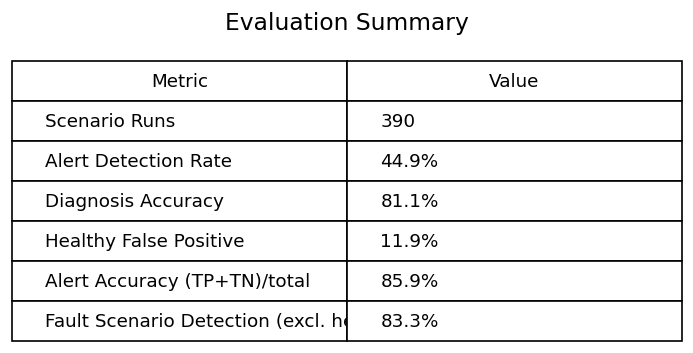
\includegraphics[width=0.65\textwidth]{00_summary_kpis}
\caption{Evaluation summary: scenario runs, detection rate, diagnosis accuracy, healthy false positive rate, fault scenario detection rate.}
\label{fig:eval_summary}
\end{figure}

\section{Alert Detection Results}

Overall detection rate across all runs is 44.9\%; excluding healthy runs, fault scenario detection rate is 83.3\%. Table~\ref{tab:detection_by_signal} and Figure~\ref{fig:detection_by_signal} show detection by signal. \texttt{bearing\_temp\_c}, \texttt{flow\_m3h}, \texttt{pressure\_bar}, \texttt{motor\_current\_a}, \texttt{valve\_flow\_mismatch}, \texttt{temp\_c}, and \texttt{rpm} achieve 100\% detection on their expected scenarios; \texttt{vibration\_rms} achieves 50\% (30 of 60 expected runs). \texttt{noise\_burst\_eval} produces no alerts (0\% detection) because the transient spike does not meet the sustained duration threshold (\texttt{min\_duration\_sec}). Healthy false positive rate is 11.9\% (25 of 210 runs); all false positives are from \texttt{bearing\_temp\_c}, likely due to ambient or startup temperature variation.

\begin{table}[htbp]
\centering
\caption{Alert detection by signal.}
\label{tab:detection_by_signal}
\small
\begin{tabular}{@{}llrr@{}}
\toprule
\textbf{Signal} & \textbf{Expected runs} & \textbf{Hits} & \textbf{Detection rate (\%)} \\
\midrule
bearing\_temp\_c & 30 & 30 & 100 \\
flow\_m3h & 30 & 30 & 100 \\
pressure\_bar & 30 & 30 & 100 \\
motor\_current\_a & 30 & 30 & 100 \\
valve\_flow\_mismatch & 30 & 30 & 100 \\
temp\_c & 30 & 30 & 100 \\
rpm & 30 & 30 & 100 \\
vibration\_rms & 60 & 30 & 50 \\
\bottomrule
\end{tabular}
\end{table}

\begin{figure}[htbp]
\centering
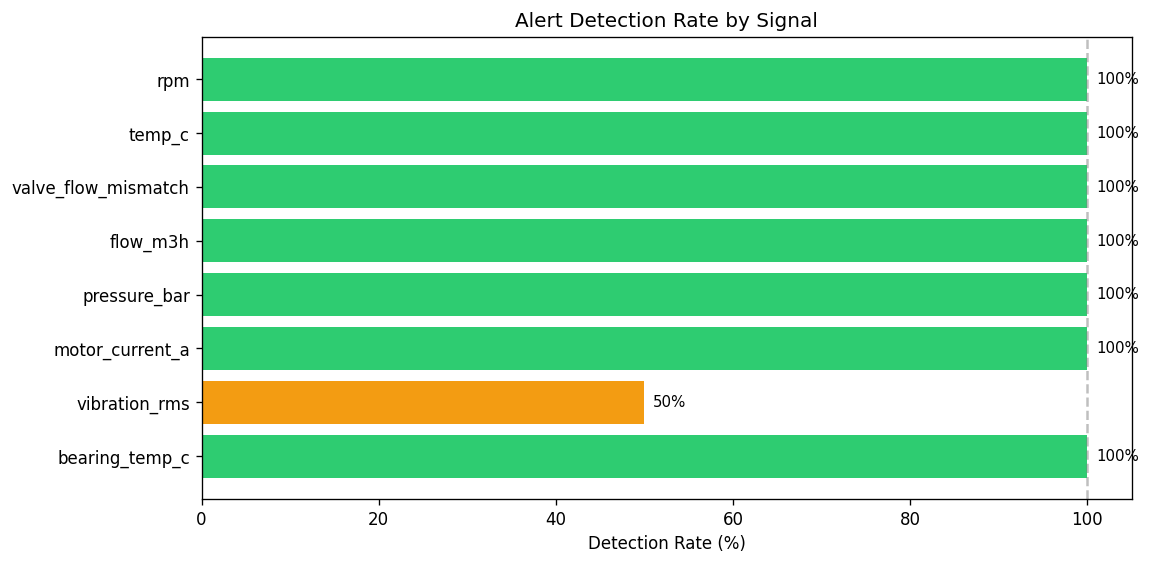
\includegraphics[width=0.9\textwidth]{01_detection_by_signal}
\caption{Alert detection rate by signal (\%).}
\label{fig:detection_by_signal}
\end{figure}

\section{Diagnosis Accuracy}

Across 196 diagnoses, 159 are correct (81.1\% accuracy). Table~\ref{tab:diagnosis_accuracy} and Figure~\ref{fig:diagnosis_accuracy} show per-root-cause accuracy. \texttt{bearing\_wear} and \texttt{valve\_stuck} achieve 100\%; \texttt{clogging} 73.7\%; \texttt{sensor\_override} 53.3\%; \texttt{none} (healthy) 66.7\%. Figure~\ref{fig:confusion_matrix} shows the confusion matrix. Clogging is confused with \texttt{valve\_stuck} and \texttt{bearing\_wear}; valve\_stuck with \texttt{clogging}; sensor\_override with \texttt{sensor\_drift}, \texttt{bearing\_wear}, and \texttt{clogging}; healthy (\texttt{none}) is misdiagnosed as \texttt{bearing\_wear}, \texttt{clogging}, or \texttt{sensor\_drift}.

\begin{table}[htbp]
\centering
\caption{Diagnosis accuracy by root cause.}
\label{tab:diagnosis_accuracy}
\small
\begin{tabular}{@{}llrr@{}}
\toprule
\textbf{Root cause} & \textbf{Count} & \textbf{Correct} & \textbf{Accuracy (\%)} \\
\midrule
bearing\_wear & 78 & 78 & 100.0 \\
valve\_stuck & 27 & 27 & 100.0 \\
clogging & 19 & 14 & 73.7 \\
sensor\_override & 60 & 32 & 53.3 \\
none & 12 & 8 & 66.7 \\
\bottomrule
\end{tabular}
\end{table}

\begin{figure}[htbp]
\centering
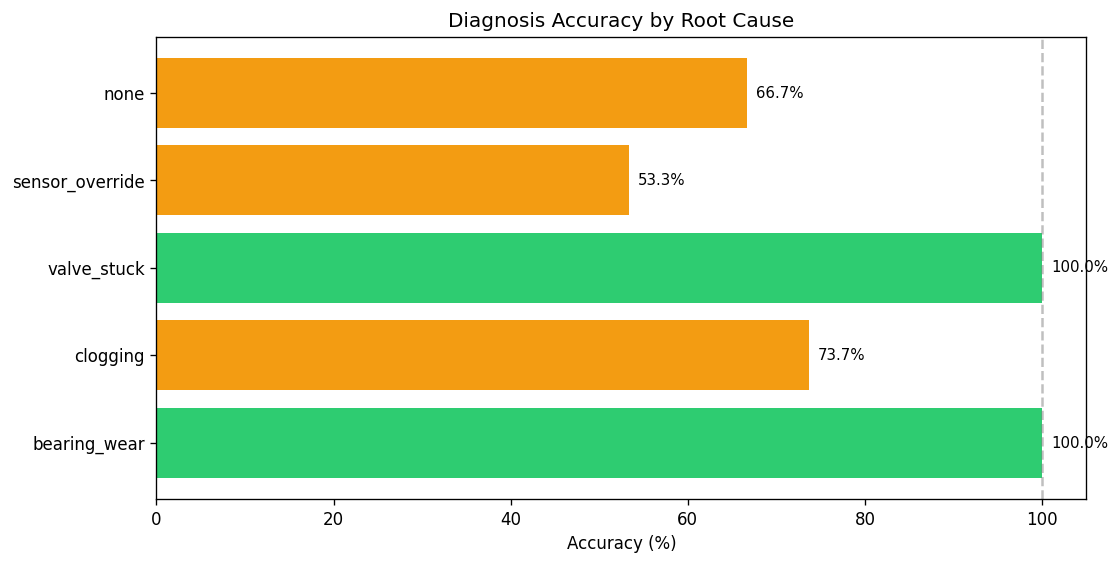
\includegraphics[width=0.9\textwidth]{02_diagnosis_accuracy}
\caption{Diagnosis accuracy by root cause (\%).}
\label{fig:diagnosis_accuracy}
\end{figure}

\begin{figure}[htbp]
\centering
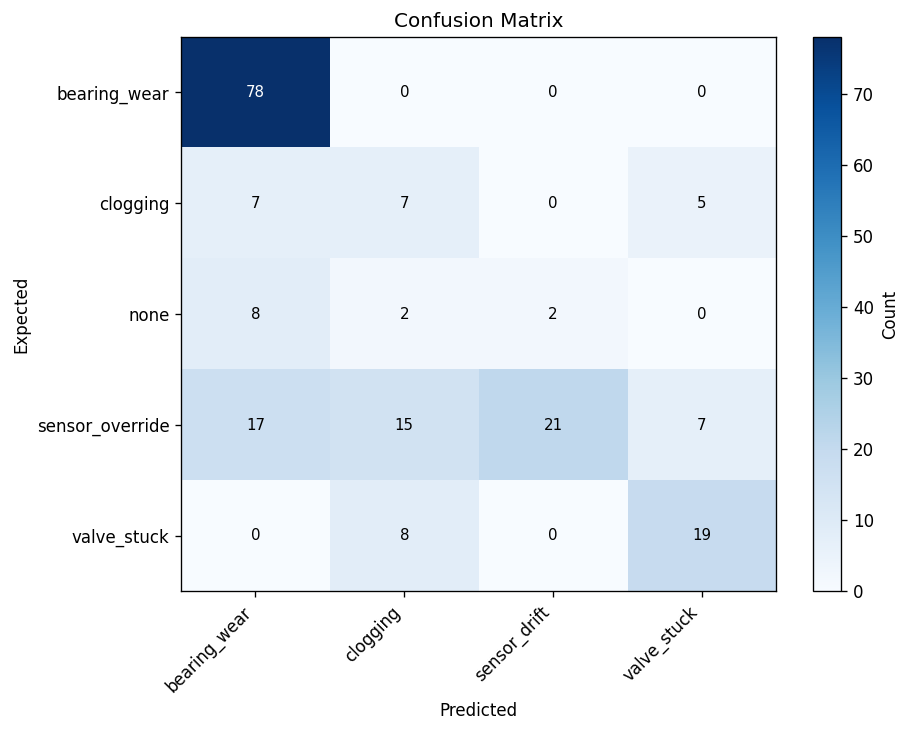
\includegraphics[width=0.75\textwidth]{06_confusion_matrix}
\caption{Confusion matrix: expected (rows) vs.\ predicted (columns).}
\label{fig:confusion_matrix}
\end{figure}

\section{Scenario Matrix}

Figure~\ref{fig:scenario_matrix} compares detection rate and diagnosis accuracy per fault scenario. \texttt{bearing\_wear\_eval} and \texttt{valve\_flow\_mismatch\_eval} achieve 100\% on both. \texttt{clogging\_eval} has 100\% detection but 73.7\% diagnosis accuracy (confusion with valve\_stuck). \texttt{sensor\_drift\_eval\_temp\_override} and \texttt{rpm\_eval\_override} have 100\% detection but lower diagnosis accuracy (63.3\% and 43.3\%). \texttt{noise\_burst\_eval} has 0\% detection, so no diagnoses are produced.

\begin{figure}[htbp]
\centering
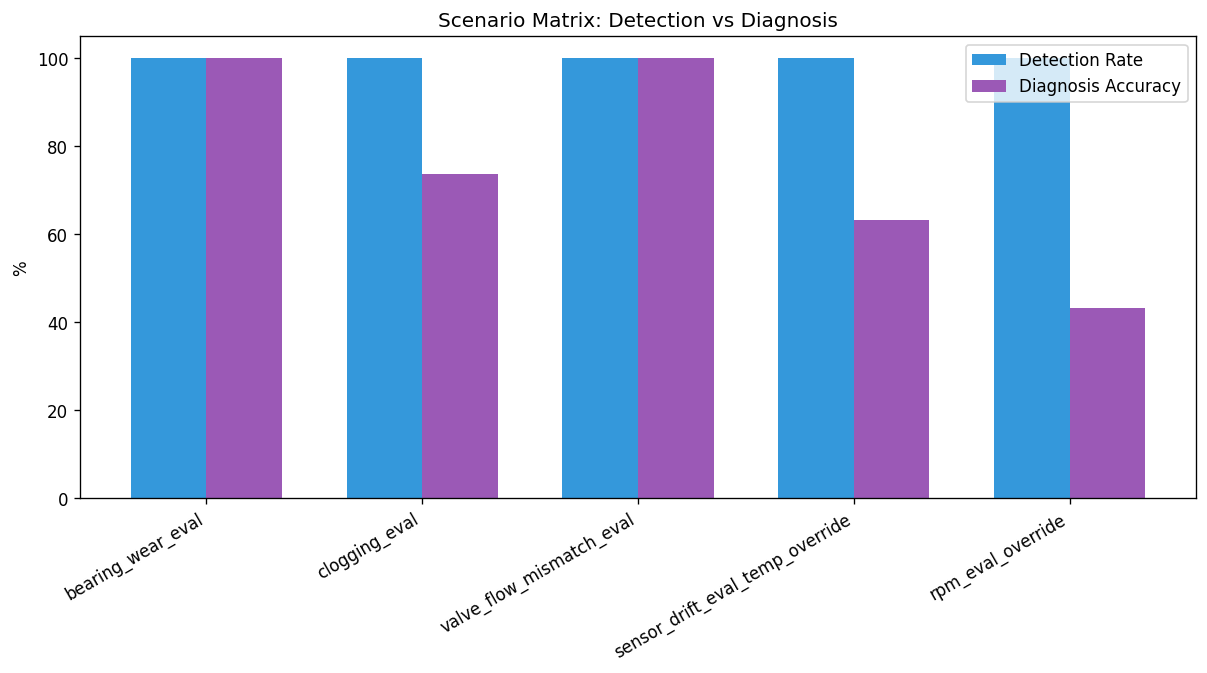
\includegraphics[width=0.95\textwidth]{03_scenario_matrix}
\caption{Scenario matrix: detection rate vs.\ diagnosis accuracy per fault scenario.}
\label{fig:scenario_matrix}
\end{figure}

\section{Token Usage and Latency}

Correct diagnoses use fewer steps (8.2 vs.\ 9.3) and fewer tokens (38.5k vs.\ 49.8k) on average than incorrect ones (Figure~\ref{fig:correct_vs_incorrect}). Figure~\ref{fig:tokens_by_scenario} shows token usage by scenario: \texttt{bearing\_wear\_eval} uses the fewest (~27.7k tokens); \texttt{clogging\_eval}, \texttt{sensor\_override} scenarios, and \texttt{healthy\_baseline} use more. Alert-to-diagnosis latency is low (avg 0.02\,s for fault scenarios); healthy false positives have higher latency (avg 0.13\,s).

\begin{figure}[htbp]
\centering
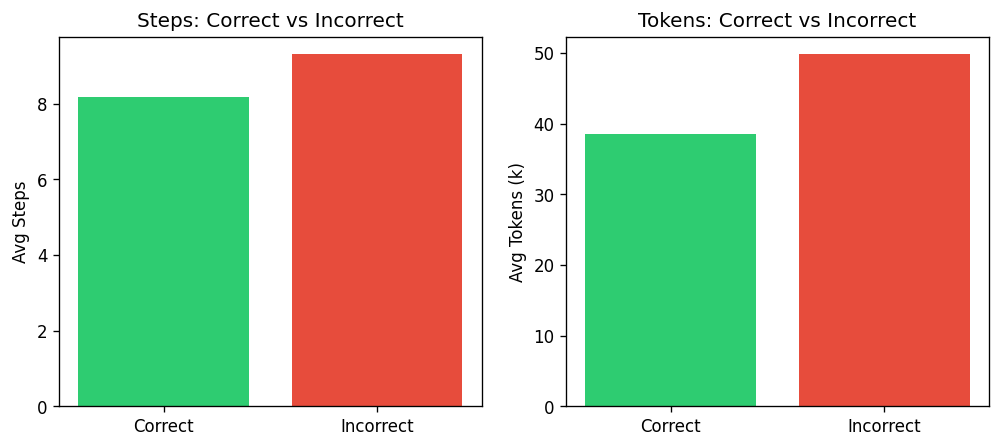
\includegraphics[width=0.9\textwidth]{04_correct_vs_incorrect}
\caption{Steps and tokens: correct vs.\ incorrect diagnoses.}
\label{fig:correct_vs_incorrect}
\end{figure}

\begin{figure}[htbp]
\centering
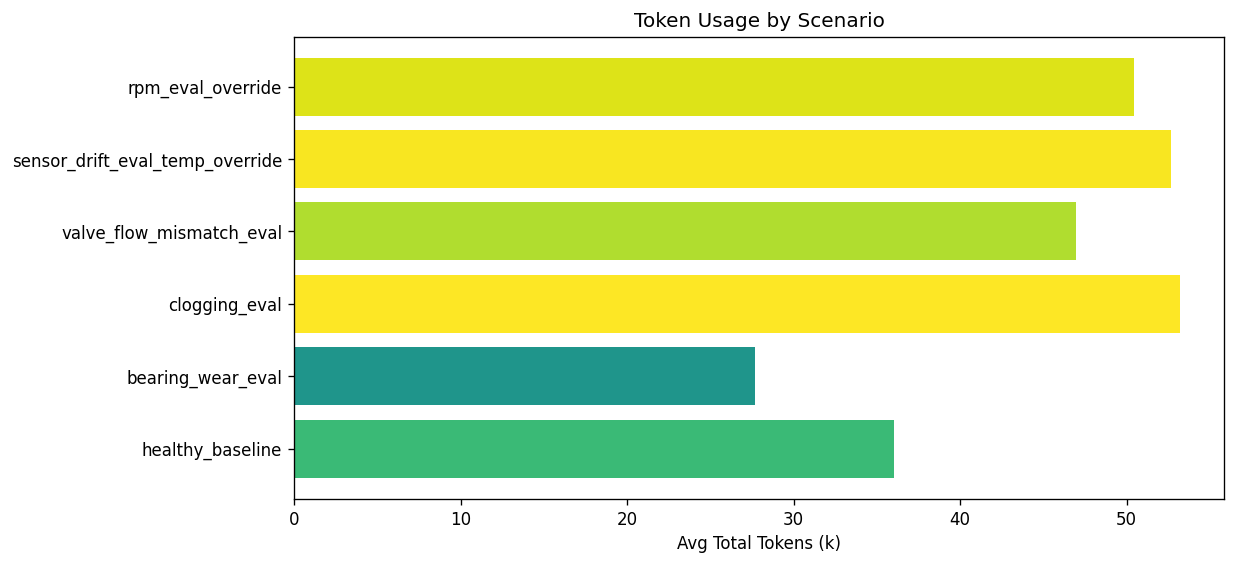
\includegraphics[width=0.9\textwidth]{05_tokens_by_scenario}
\caption{Average token usage by scenario (k tokens).}
\label{fig:tokens_by_scenario}
\end{figure}

\section{Discussion}

Strengths include high accuracy for bearing wear and valve stuck (100\%), interpretable evidence (ReAct reasoning and rule retrieval), and reproducible evaluation (fixed scenarios, JSONL logs, DB queries). Limitations include: (1) \texttt{noise\_burst} detection failure (0\%) because transient spikes do not meet duration thresholds; (2) confusion between clogging and valve\_stuck (both affect flow and valve); (3) sensor\_override confusion with bearing\_wear and clogging (LLM struggles to distinguish sensor faults from real faults); (4) healthy false positives from \texttt{bearing\_temp\_c}, suggesting threshold tuning or startup filtering.

\section{Improvement Opportunities}

Alert detection: tune thresholds or reduce \texttt{min\_duration\_sec} for transient spikes (\texttt{noise\_burst}); add startup cooldown to reduce bearing\_temp\_c false positives on healthy runs. Diagnosis: add discriminative rules for clogging vs.\ valve\_stuck (e.g., slope of flow vs.\ valve position); improve rules for sensor\_override vs.\ bearing\_wear. RAG: batch indexing, hybrid keyword-semantic search. Future work: real sensor data, multi-asset scaling, improved noise\_burst detection.

% ========== Chapter 6: Conclusion ==========
\chapter{Conclusion}
\label{ch:conclusion}

\section{Summary}

This report presented the design, implementation, and evaluation of a multi-agent powerplant monitoring system. The architecture comprises four agents (Monitor, Diagnosis, Ticket, Review) communicating via MQTT, with separation of concerns for scalability and fault isolation. Agent A uses threshold-based and slope-based detection for real-time anomaly alerts; Agent B performs root cause diagnosis via ReAct with tool-augmented LLMs~\cite{yao2023react,schick2023toolformer} and rule retrieval; Agent C creates review requests; Agent D provides a human-in-the-loop interface with RAG-assisted chat~\cite{lewis2020rag}, approve/reject workflow, and optional Salesforce Case creation. A physics-based simulator with fault injection (bearing wear, clogging, valve stuck, sensor drift, noise burst) enables reproducible evaluation.

Evaluation on 390 scenario runs showed 81.1\% diagnosis accuracy with 100\% for bearing wear and valve stuck, 83.3\% fault scenario detection rate, and 11.9\% healthy false positive rate. Correct diagnoses use fewer ReAct steps and tokens than incorrect ones; the confusion matrix reveals that sensor\_override and clogging are the most challenging fault types. The system demonstrates that a rule-plus-LLM hybrid diagnosis approach with evidence traceability can achieve reliable fault diagnosis for well-defined fault types while maintaining interpretability. A key contribution of this work is the effectiveness of the rule-plus-LLM hybrid for industrial fault diagnosis, combining interpretable rule retrieval with LLM reasoning and tool use.

\section{Future Work}

Future work includes: (1) \textbf{Vision integration}---enable VLM analysis of 3D pump renderings and dashboard screenshots for visual anomaly detection; (2) \textbf{Multi-asset scaling}---extend the pipeline to multiple pumps and assets with per-asset or shared models; (3) \textbf{Improved noise\_burst detection}---tune thresholds or reduce \texttt{min\_duration\_sec} for transient spikes, or add a dedicated short-window detector; (4) \textbf{Real sensor data evaluation}---validate on industrial telemetry from physical pumps or test rigs; (5) \textbf{RAG enhancements}---batch indexing, hybrid keyword-semantic search, and retrieval quality tuning; (6) \textbf{Discriminative rules}---add rules to better distinguish clogging vs.\ valve\_stuck and sensor\_override vs.\ bearing\_wear.

% ========== References ==========
\singlespacing
\bibliographystyle{ieeetr}
\bibliography{references}
\doublespacing

% ========== Appendices ==========
\appendix
\chapter{Database Schema}
\label{app:db_schema}

The schema is created by \texttt{scripts/init\_db.py}. Indexes on \texttt{(asset\_id, ts)} and \texttt{(ts, asset\_id)} support time-range queries. The \texttt{vec\_memory} virtual table is created when sqlite-vec is installed (Section~4.6). Tables are listed below with column descriptions.

\subsection*{telemetry}
Source: Simulator. Sensor readings per timestamp.

\begin{tabular}{@{}llp{5.5cm}@{}}
\toprule
\textbf{Column} & \textbf{Type} & \textbf{Description} \\
\midrule
id & INTEGER PK & Auto-increment primary key \\
ts & TEXT & Timestamp (ISO) \\
plant\_id & TEXT & Plant identifier \\
asset\_id & TEXT & Asset identifier (e.g.\ pump01) \\
pressure\_bar & REAL & Pressure (bar) \\
flow\_m3h & REAL & Flow (m$^3$/h) \\
temp\_c & REAL & Temperature (°C) \\
bearing\_temp\_c & REAL & Bearing temperature (°C) \\
vibration\_rms & REAL & Vibration RMS (mm/s) \\
rpm & REAL & Rotational speed \\
motor\_current\_a & REAL & Motor current (A) \\
valve\_open\_pct & REAL & Valve opening (\%) \\
fault & TEXT & Injected fault type (default: none) \\
severity & REAL & Fault severity \\
created\_at & TEXT & Row creation time \\
\bottomrule
\end{tabular}

\subsection*{alerts}
Source: Agent A. Anomaly alerts from threshold/slope detection.

\begin{tabular}{@{}llp{5.5cm}@{}}
\toprule
\textbf{Column} & \textbf{Type} & \textbf{Description} \\
\midrule
id & INTEGER PK & Auto-increment primary key \\
ts & TEXT & Alert timestamp \\
plant\_id, asset\_id & TEXT & Plant and asset identifiers \\
severity & TEXT & warning, critical \\
signal & TEXT & Signal that triggered (e.g.\ bearing\_temp\_c) \\
score & REAL & Severity score \\
method & TEXT & threshold, slope, valve\_flow\_mismatch \\
evidence & TEXT & JSON: value, threshold, duration \\
created\_at & TEXT & Row creation time \\
\bottomrule
\end{tabular}

\subsection*{diagnosis}
Source: Agent B. Root cause diagnosis from ReAct agent.

\begin{tabular}{@{}llp{5.5cm}@{}}
\toprule
\textbf{Column} & \textbf{Type} & \textbf{Description} \\
\midrule
id & INTEGER PK & Auto-increment primary key \\
ts & TEXT & Diagnosis timestamp \\
plant\_id, asset\_id & TEXT & Plant and asset identifiers \\
alert\_id & INTEGER & FK to alerts (optional) \\
root\_cause & TEXT & bearing\_wear, clogging, valve\_stuck, sensor\_drift, unknown \\
confidence & REAL & 0--1 \\
impact & TEXT & low, medium, high \\
recommended\_actions & TEXT & JSON array \\
evidence & TEXT & JSON array of rule references \\
recursion\_limit, actual\_steps & INTEGER & ReAct steps (eval) \\
total\_tokens, prompt\_tokens, completion\_tokens & INTEGER & Token counts (eval) \\
created\_at & TEXT & Row creation time \\
\bottomrule
\end{tabular}

\subsection*{vision\_images}
Source: Simulator. Paths to 3D renderings or screenshots.

\begin{tabular}{@{}llp{5.5cm}@{}}
\toprule
\textbf{Column} & \textbf{Type} & \textbf{Description} \\
\midrule
id & INTEGER PK & Auto-increment primary key \\
ts & TEXT & Timestamp \\
plant\_id, asset\_id & TEXT & Plant and asset identifiers \\
image\_path & TEXT & File path to image \\
created\_at & TEXT & Row creation time \\
\bottomrule
\end{tabular}

\subsection*{vision\_analysis}
Source: Agent D (VLM). VLM analysis results for images.

\begin{tabular}{@{}llp{5.5cm}@{}}
\toprule
\textbf{Column} & \textbf{Type} & \textbf{Description} \\
\midrule
id & INTEGER PK & Auto-increment primary key \\
ts & TEXT & Timestamp \\
plant\_id, asset\_id & TEXT & Plant and asset identifiers \\
image\_path & TEXT & Path to analyzed image \\
description & TEXT & VLM description \\
anomalies\_detected & TEXT & Detected anomalies \\
confidence & REAL & VLM confidence \\
created\_at & TEXT & Row creation time \\
\bottomrule
\end{tabular}

\subsection*{tickets}
Source: Agent D. External tickets (Salesforce Case, GitHub Issue) created on approve.

\begin{tabular}{@{}llp{5.5cm}@{}}
\toprule
\textbf{Column} & \textbf{Type} & \textbf{Description} \\
\midrule
id & INTEGER PK & Auto-increment primary key \\
ts & TEXT & Creation timestamp \\
plant\_id, asset\_id & TEXT & Plant and asset identifiers \\
ticket\_id & TEXT UNIQUE & External system ID (e.g.\ Case Id) \\
title & TEXT & Ticket title \\
body & TEXT & Ticket description \\
status & TEXT & open, closed (default: open) \\
diagnosis\_id & INTEGER & FK to diagnosis \\
url & TEXT & Link to external record (e.g.\ Lightning URL) \\
created\_at & TEXT & Row creation time \\
\bottomrule
\end{tabular}

\subsection*{review\_requests}
Source: Agent C. Queue of diagnoses awaiting human review.

\begin{tabular}{@{}llp{5.5cm}@{}}
\toprule
\textbf{Column} & \textbf{Type} & \textbf{Description} \\
\midrule
id & INTEGER PK & Auto-increment primary key \\
diagnosis\_id & INTEGER & FK to diagnosis \\
plant\_id, asset\_id & TEXT & Plant and asset identifiers \\
ts & TEXT & Timestamp \\
status & TEXT & pending, approved, rejected (default: pending) \\
created\_at & TEXT & Row creation time \\
resolved\_at & TEXT & When status was updated \\
\bottomrule
\end{tabular}

\subsection*{chat\_sessions}
Source: Agent D. Chat conversation sessions.

\begin{tabular}{@{}llp{5.5cm}@{}}
\toprule
\textbf{Column} & \textbf{Type} & \textbf{Description} \\
\midrule
id & INTEGER PK & Auto-increment primary key \\
created\_at, updated\_at & TEXT & Session timestamps \\
preview & TEXT & Preview of last message \\
\bottomrule
\end{tabular}

\subsection*{chat\_messages}
Source: Agent D. Messages within a chat session.

\begin{tabular}{@{}llp{5.5cm}@{}}
\toprule
\textbf{Column} & \textbf{Type} & \textbf{Description} \\
\midrule
id & INTEGER PK & Auto-increment primary key \\
session\_id & INTEGER & FK to chat\_sessions \\
role & TEXT & user, assistant \\
content & TEXT & Message text \\
tool\_calls & TEXT & JSON of tool calls (assistant) \\
created\_at & TEXT & Row creation time \\
\bottomrule
\end{tabular}

\subsection*{chat\_steps}
Source: Agent D. ReAct steps (thought, tool\_call, tool\_result) per message.

\begin{tabular}{@{}llp{5.5cm}@{}}
\toprule
\textbf{Column} & \textbf{Type} & \textbf{Description} \\
\midrule
id & INTEGER PK & Auto-increment primary key \\
message\_id & INTEGER & FK to chat\_messages \\
step\_type & TEXT & thought, tool\_call, tool\_result \\
step\_order & INTEGER & Order within message \\
tool\_name & TEXT & Tool name (if tool\_call) \\
tool\_args & TEXT & JSON args (if tool\_call) \\
content & TEXT & Step content \\
raw\_result & TEXT & Tool output (if tool\_result) \\
created\_at & TEXT & Row creation time \\
\bottomrule
\end{tabular}

\subsection*{feedback}
Source: Agent D. Human review decisions (approve/reject) with notes.

\begin{tabular}{@{}llp{5.5cm}@{}}
\toprule
\textbf{Column} & \textbf{Type} & \textbf{Description} \\
\midrule
id & INTEGER PK & Auto-increment primary key \\
ts & TEXT & Timestamp \\
plant\_id, asset\_id & TEXT & Plant and asset identifiers \\
ticket\_id & TEXT & Associated ticket ID \\
review\_decision & TEXT & approved, rejected, edited \\
final\_root\_cause & TEXT & Reviewer-confirmed root cause \\
notes & TEXT & Reviewer notes \\
created\_at & TEXT & Row creation time \\
\bottomrule
\end{tabular}

\subsection*{vec\_memory (virtual table)}
Source: sqlite-vec extension. RAG vector store (384-dim embeddings).

\begin{tabular}{@{}llp{5.5cm}@{}}
\toprule
\textbf{Column} & \textbf{Type} & \textbf{Description} \\
\midrule
embedding & float[384] & Dense embedding (all-MiniLM-L6-v2) \\
metadata & TEXT & JSON: doc\_type, doc\_id, asset\_id, text preview \\
\bottomrule
\end{tabular}

\chapter{Scenario JSON Example}
\label{app:scenario_json}

Scenario definitions are stored as JSON files in \texttt{simulator-service/scenarios/}. The Simulator loads a scenario by name and executes the simulation loop with the specified faults, initial conditions, and setpoints. Listing~\ref{lst:scenario_bearing} shows \texttt{bearing\_wear\_eval.json}: a fault scenario that injects bearing wear from the start with \texttt{rate\_per\_sec}=0.35. Listing~\ref{lst:scenario_healthy} shows \texttt{healthy\_baseline.json}: no faults, with setpoints that change valve opening at 200\,s and 400\,s.

\begin{lstlisting}[language=Python, caption={bearing\_wear\_eval.json}, label=lst:scenario_bearing, breaklines=true]
{
  "version": "1.0",
  "name": "bearing_wear_eval",
  "description": "Fast bearing wear for eval - triggers vibration/bearing_temp slope + threshold alerts",
  "plant_id": "plant01",
  "asset_id": "pump01",
  "seed": 12345,
  "duration_sec": 300,
  "initial_conditions": { "rpm": 2950, "valve_open_pct": 60 },
  "faults": [{ "type": "bearing_wear", "start_time_sec": 0, "params": { "rate_per_sec": 0.35 } }],
  "setpoints": []
}
\end{lstlisting}

\begin{lstlisting}[language=Python, caption={healthy\_baseline.json}, label=lst:scenario_healthy, breaklines=true]
{
  "version": "1.0",
  "name": "healthy_baseline",
  "description": "Healthy pump operation with no faults",
  "plant_id": "plant01",
  "asset_id": "pump01",
  "seed": 12345,
  "duration_sec": 600,
  "initial_conditions": { "rpm": 2950, "valve_open_pct": 60.0 },
  "faults": [],
  "setpoints": [
    { "time_sec": 200, "valve_open_pct": 70.0 },
    { "time_sec": 400, "valve_open_pct": 50.0 }
  ]
}
\end{lstlisting}

\chapter{Rule Document Example}
\label{app:rule_doc}

Diagnosis rules are stored as Markdown files in \texttt{agent-diagnosis/rules/}. Agent B's \texttt{query\_rules} tool searches these files by keyword and returns matching content. The agent uses \texttt{compute\_slope} to confirm trends suggested by the rules. Listing~\ref{lst:rule_bearing} shows \texttt{bearing\_wear.md}.

\begin{lstlisting}[language=Python, caption={bearing\_wear.md (agent-diagnosis/rules/)}, label=lst:rule_bearing, breaklines=true]
# Bearing Wear

## Root Cause
bearing_wear

## Symptoms
- Elevated vibration_rms (above baseline)
- Elevated bearing_temp_c (above ambient + normal load)
- May accompany minor rpm fluctuation or motor_current_a increase

## Related Signals
vibration_rms, bearing_temp_c, rpm, motor_current_a

## Variants
- **Chronic**: vibration slope > 0 over 60s, sustained > 30s (gradual degradation)
- **Acute**: vibration + bearing_temp both above threshold, slope positive (rapid onset)

## Recommended Actions
- Check bearing lubrication level and quality
- Inspect bearing for wear, pitting, or contamination
- Schedule planned shutdown for bearing replacement if degradation confirmed
- Monitor vibration trend to assess progression

## Time/Trend Hints
- Use compute_slope(asset_id, "vibration_rms", 60) to check for gradual increase
- Use compute_slope(asset_id, "bearing_temp_c", 60) for temperature trend
- Chronic bearing wear: slope > 0 over 60s, sustained > 30s
- Acute: both signals above threshold with positive slope

## Impact
High - can lead to catastrophic failure if unaddressed
\end{lstlisting}

% ========== Project Links ==========
\chapter{Project Links}
\label{app:project_links}

The full project code and a live demo deployment are publicly available:

\begin{itemize}
  \item \textbf{GitHub repository}: \url{https://github.com/Haoj1/Powerplant-Multi-Agent}
  \item \textbf{Live demo (Agent D Review Dashboard)}: \url{https://app.powerplantagent.com/review}
\end{itemize}

The GitHub repository includes installation instructions, quickstart scripts, evaluation tooling, and additional architecture documentation. The live demo exposes the Review dashboard (Review Queue, Alerts, Sensors, Chat, and Scenarios) backed by the same multi-agent system described in this report.

\end{document}
